%\documentclass[10pt,conference]{IEEEtran}
\documentclass[sigconf,review, anonymous]{acmart}
\acmConference[ISSTA 2023]{ACM SIGSOFT International Symposium on Software Testing and Analysis}{17-21 July, 2023}{Seattle, USA}
%\IEEEoverridecommandlockouts


% Fonte em português brasileiro
\usepackage[american]{babel}
\usepackage[utf8]{inputenc}
\usepackage{enumerate}
\usepackage{pgfgantt}
\usepackage{booktabs}
\usepackage{listings}
\usepackage{hyperref}
\usepackage{xspace}
\usepackage{balance}
\usepackage{parselines}
\usepackage{comment}
\usepackage[most]{tcolorbox}
\usepackage{pgfplotstable}
\usepackage{awesomebox}



% Custom colors
\definecolor{keywords}{rgb}{0.5,0,0.35}
\definecolor{comments}{RGB}{0,0,113}
\definecolor{red}{RGB}{160,0,0}
\definecolor{green}{RGB}{0,150,0}
 
\lstset{language=Python, 
        basicstyle=\ttfamily\small, 
        keywordstyle=\color{keywords}\bfseries,
        commentstyle=\color{comments},
        stringstyle=\color{red},
        showstringspaces=false,
        %identifierstyle=\color{red},
       }
       


% Pictures
\usepackage{graphicx}       

\def\BibTeX{{\rm B\kern-.05em{\sc i\kern-.025em b}\kern-.08em
    T\kern-.1667em\lower.7ex\hbox{E}\kern-.125emX}}

\newtcbtheorem{obs}{Finding}{%
        theorem name,%
        colback=gray!5,%
        colframe=gray!35!black,%
        fonttitle=\bfseries,title after break={Lemma  -- \raggedleft Continued}%
    }{lem}

\newcommand{\tb}[2]{\tipbox{{\bf Finding #1}. #2}}

\newcommand{\droidxp}{DroidXP\xspace}

\newcommand\kn[1]{\textcolor{red}{KN: #1}}
\newcommand\fh[1]{\textcolor{green}{FH: #1}}
\newcommand\rb[1]{(\textcolor{blue}{RB: #1})}

\newcommand{\highlight}[1]{{\color{red}}#1}

\newcommand\raw[1]{\textcolor{red}{#1}\xspace}

\newcommand{\mas}{MAS approach\xspace}

\newcommand{\fm}[1]{\emph{#1}\xspace}

\newcommand{\gps}{\fm{gappusin}\xspace}  % the gappusin family.

\newcommand{\sscore}{Similarity Score\xspace}

\newcommand{\rqa}{What is the impact of a more diverse dataset on the accuracy of the \mas for malware detection?}

\newcommand{\rqb}{How much gain we obtain on the performance of the \mas for malware detection when considering trace analysis?}

\newcommand{\rqc}{What is the influence of the similarity between the original and repackaged
                  versions of the apps on the performance of the \mas for malware detection?}

\newcommand{\rqd}{What is the influence of the malware family on the performance of the \mas for malware detection?}


\newcommand{\appsSmall}{102\xspace}
\newcommand{\apps}{1,707\xspace}

\newcommand{\sds}{\texttt{Small Dataset}\xspace}
\newcommand{\cds}{\texttt{Complete Dataset}\xspace}
\newcommand{\avt}{\texttt{avclass2} tool\xspace}
\newcommand{\vt}{\texttt{VirusTotal}\xspace}
\newcommand{\se}{security engine\xspace}
\newcommand{\ses}{security engines\xspace}


\newcommand{\fscoreSmall}{0.89\xspace}
\newcommand{\fscore}{0.33\xspace}

\newcommand{\malwares}{490\xspace}
\newcommand{\malwaresP}{28.70}
\newcommand{\appsGps}{\raw{295}}
\newcommand{\appsGpsFN}{\raw{269}}

\setlength {\marginparwidth }{2cm}
\pgfplotsset{compat=1.18}

\title{The Achilles' Heel of the Android Mining Sandbox Approach for Malware Identification (Replicability Studies)}

\begin{document}



% Title Alternatives
% - \title{The Achilles' Heel of the Mining Sandbox Approach for Android Malware Identification}
% - ...
% 
% Here we will put author ...

%\author{Francisco Costa}
%\affiliation{%
%  \institution{Brasilia University}
%  \city{Brasilia}
%  \country{Brazil}}
%\email{180040723@aluno.unb.br}





\IEEEtitleabstractindextext{
\begin{abstract}
The widespread use of smartphones in our daily lives has elevated concerns regarding their security among researchers and practitioners.
Particularly, security issues are highly prevalent in Android, the most popular mobile operating system. Previous research has explored
various techniques to address these concerns, including the Mining Android Sandbox approach (\mas), which aims to identify malicious behavior in repackaged Android applications (apps).
However, earlier studies have been limited by small datasets, typically consisting of only \appsSmall pairs of original and repackaged apps.
This limitation raises questions about the external validity of their findings and whether the MAS approach is scalable to larger datasets.
To address these concerns, this paper presents the results of an experiment that replicates state-of-the-art research on evaluating the
accuracy of the \mas. Unlike previous studies, our research employs a dataset that is an order of magnitude larger, comprising \apps
pairs of apps covering a more diverse range of Android malware families. Surprisingly, our findings indicate a significant drop in the accuracy of the MAS approach for identifying malware, with
the \fone decreasing from \fscoreSmall in previous studies to \fscore in our larger dataset.
Upon closer examination, we discovered that the higher representation of malware from the gappusin family partially accounts for the increased
number of instances where the \mas fails to correctly classify a repackaged app as malware. Additionally, we investigated the impact of two extensions—--Trace Analysis and Parameter Analysis—implemented
from the literature to enhance the \mas. However, these extensions only marginally improved the approach's performance, with both extensions combined increasing accuracy by 8\%
(from 52\% to 60\%)—--still falling short of the accuracy reported in previous studies.
Our findings highlight the limitations of the MAS approach, particularly when scaled, and underscore the importance of complementing it with other techniques to effectively detect a
broader range of malware. This opens avenues for further discussion on addressing the blind spots
that affect the accuracy of the MAS approach.
\end{abstract}
}

%\begin{IEEEkeywords}
%  Android Malware Detection, Dynamic Analysis, Mining Android Sandboxes
%\end{IEEEkeywords}

\keywords{Android Malware Detection, Dynamic Analysis, Mining Android Sandboxes}
\maketitle
\section{Introduction}\label{sec:introduction}

Mobile technologies like smartphones and tablets have become fundamental to the way we function as a society. Almost two-thirds of the world population
uses mobile technologies~\cite{Comscore,DBLP:journals/tse/MartinSJZH17}, with the
Android Platform dominating this market and accounting for more than 70\% of the \emph{mobile
market share} with almost 3.5 million Android applications~\footnote{In this paper, we will use the terms Android Applications, Android Apps, and Apps interchangeably, to refer to Android software applications} (apps)
available on the Google Play Store~\cite{Statista}. 
With increased popularity, comes increased risk of attacks---motivating efforts from both academia and industry to design and develop new techniques
to identify malicious behavior or vulnerable code in Android apps~\cite{10.1145/3017427}.


One of the most popular classes of malwares are based on repackaging apps~\cite{DBLP:conf/wcre/BaoLL18,le2018towards} where benign
versions of an app from an official app store are
%such as Google Play, 
infected with malicious code, e.g., to broadcast
sensitive information to a private server~\cite{DBLP:journals/tse/LiBK21}, and subsequently shared
with users using different app stores.  The focus of this paper is the Mining Android Sandbox, hereafter \mas, which has been shown effective
in detecting the popular class of Android malware based on 
repackaging benign apps. 
It  takes advantage of automated test case generation tools 
to explore the behavior of an app---in terms of calls to sensitive APIs---and then
generates a sandbox~\cite{DBLP:conf/icse/JamrozikSZ16}. During a normal
execution of the app, the sandbox might block calls to a sensitive API
that had not been observed during the exploratory phase. 


Previous studies~\cite{DBLP:conf/wcre/BaoLL18,DBLP:journals/jss/CostaMMSSBNR22} 
have compared the accuracy of  Android sandboxes for malware detection 
that were produced 
from 
%executing 
different test case generation tools, including Monkey~\cite{Monkey}, DroidBot~\cite{DBLP:conf/icse/LiYGC17}, and Droidmate~\cite{DBLP:conf/kbse/BorgesHZ18} tools.
The studies bring evidence that 
DroidBot outperforms the other test generation tools and leads to sandboxes that are more accurate in detecting malware with a classification rate of 70\%.
But these previous studies have two main limitations.
First, they use a small dataset of malware comprising only \appsSmall pairs of original/repackaged versions of an app. This decision
might compromise the external validity of previous studies. Second, their assessment do not investigate
the impact of repackaged characteristics on the accuracy of the \mas for malware classification, including
(a) whether or not the repackaged version is a malware, (b) the similarity between the original and the repackaged versions of an app,
and (c) the malware family (e.g., \fm{gappusin}, \fm{kuguo}, \fm{dowgin}, etc.) when the repackaged
version of an app is a malware.

%{\bf MM: The second part of the last sentence is not clear. Are similarity and malware family two different "malware characteristics"?}

%In this paper, we present the results of an investigation that aims to replicate previous studies~\cite{DBLP:conf/wcre/BaoLL18,DBLP:conf/scam/CostaMCMVBC20} in a larger dataset of app pairs (original/repackaged versions), and then explore whether a more diverse sample of app pairs has an influence on the accuracy of the \mas for malware identification. To this end, we explore the performance of the \mas using a larger dataset we curated for this research and DroidBot~\cite{DBLP:conf/icse/LiYGC17} as test case generation---the tool that, according to the literature, leads to the most accuracy Android sandbox. Our new dataset is an order of magnitude larger (it contains \apps pairs of original/repackaged apps), comprises a much more diverse similarity index, and covers a broader range of malware families. 

To empirically study the impact of these limitations on the reported results, in this paper we reconsider the performance of the \mas based on
DroidBot~\cite{DBLP:conf/icse/LiYGC17}---as we mentioned, the test case generation tool that, according to the literature, leads to the most accurate Android sandbox. 
Compared to previous studies~\cite{DBLP:conf/wcre/BaoLL18,DBLP:conf/scam/CostaMCMVBC20},
we use a curated dataset of app pairs (original/repackaged versions) that is, in terms of magnitude, larger than the previously used
dataset (it contains \apps pairs of original/repackaged apps).
 
{\bf Negative results.} Our study reveals a significantly lower
%on a larger and more diverse dataset (compared to previous studies), 
accuracy ($F_1$ score) of the \mas in comparison to what has been reported before (\fscore versus \fscoreSmall). 
An accuracy of \fscore is clearly unsatisfactory for a trustworthy malware classification technique.
This result motivated us to conduct a series of experiments 
to understand the reasons for the lower accuracy in our larger dataset, \textcolor{blue}{and a possible solution to revert it.}
%The original approach classifies an app as malware whenever there exists a difference between the sets of calls to sensitive APIs collected when running the test case generation tool over the original and repackaged versions of the same app.
First, we check the impact of the similarity between original and repackaged versions of
an app on the performance of the \mas for malware classification. Our results reveal a non significant association association between similarity and the accuracy of the \mas. 
%\kn{Saying there is no association is not the same as saying that similarity does not impact the accuracy. Somehow I feel this statement is very strong. I would rather say that we did not find any significant association between similarity and the accuracy of the \mas.
Second, we explore if the
malware family could explain the lower performance of the \mas for malware classification in 
our dataset.

Considering this second analysis, our results reveal that the \mas fails to correctly classify most of the samples from
the \gps malware family (a particular class of adware that frequently appears in repackaged apps). 
Out of the total of \appsGps samples within this family in our large dataset, the \mas failed to correctly classify \appsGpsFN samples as malware (false negative).
Our results reveal that this particular family is responsible for substantially reducing the recall of the \mas.
Our findings have two main implications, which open the discussion (a) on one important feature found at \gps malware family that should be
considered when building malware detection approaches that mine sandboxes, and (b) on the need to have a representative dataset, that should be labeled with sought
answers and which should leads close to real-life scenarios.
  

%{\bf MM: How is the last sentence different from the one preceding it? It appears to repeat what was just said, IMHO. Also, given that we highlight two distinguishing characteristics of the larger dataset -- similarity of apps and different malware -- I was expecting that we analyse the impact of both the diversity of apps and malware. But we report only that one particular kind of malware is responsible. The dissimilarity of app pairs has no effect? What about other families of malware?}
%

%{\bf MM: I don't get the logical implication that "Still" suggests. Also, (a) and (b) appear out of nowhere... how do they relate to what has been said before in the paragraph? What is blindspot that you are talking about here? How resp. from where do you derive the need to investigate further sources of information?}

The remainder of this paper is organized as follows. 
We provide background information on the \mas and the \mas for malware detection in
Section~\ref{sec:background}. Section~\ref{sec:experimentalSetup}
characterizes our experiments in terms of research goal, questions, metrics, datasets, and our procedures for data collection and data analysis. \textcolor{blue}{Section~\ref{sec:results}, Section~\ref{sec:resultsTraceParameter} and Section~\ref{sec:discussion} present the main findings of our experiments, results of others techniques that can complement the \mas, and possible threats to the validity of our results.} Finally,
Section~\ref{sec:conclusions} presents concluding remarks and possible future
work. The main artifacts we produced during this research are available in the
paper repository.

\begin{small}
  \begin{center}
    \url{https://anonymous.4open.science/r/paper-droidxptrace-results-F55A/}
  \end{center}
\end{small}

\section{Background and Related Work}\label{sec:background}

%% In this section, we introduce the concepts and terminology that are necessary to understand the reminder of this paper. First, Section~\ref{sec:sand} introduces some background information about \emph{sandboxes} within the security context. Section~\ref{sec:repackage} presents background information about repackaged application and how they introduce malicious behavior.
%% Finally, in Section~\ref{sec:android-sandbox} we review the \emph{mining sandbox approach} for detecting repackaged Android apps.

The Android bytecode language~\cite{DBLP:conf/issta/WangGMC15} favors reverse engineering tasks. That is, software developers can easily reverse-engineer real apps (benign), modify their contents by inserting malicious code (malware), repackage them with the malicious payloads, and re-publish them in app stores, including the Google Play Store. Repackaged Android apps can leverage the popularity of real apps, to increase its propagation and spread malware.  
Repackaging has been raised as a noteworthy security concern in Android ecosystem by stakeholders in the app development industry and researchers. Indeed, there are reports claiming that about 25\% of Google Play Store app content correspond to repackaged apps~\cite{DBLP:conf/sigmetrics/ViennotGN14}. Nevertheless, all the workload to detect and remove malware from markets by the stores (official and non-official ones), have not been accurate enough to address the problem. As a result, repackaged Android apps threaten security and privacy of unsuspicious Android app users, beyond compromising the copyright of the original developer~\cite{DBLP:journals/access/KimLCP19}. Aiming at
mitigating this threat, several techniques based on both static and dynamic analysis of Android apps have been proposed.


\subsection{Mining Android Sandboxes}\label{sec:android-sandbox}

A \emph{sandbox}
is a well-known mechanism to secure a system and forbid a software component from accessing
resources without appropriate permissions. Sandboxes have also been used to build an isolated
environment within which applications cannot affect other programs, the network, or other device data~\cite{DBLP:journals/peerj-cs/MaassSCS16}. The idea of using sandboxes emerged from the
need to test unsafe software, possible malware, without worrying about the integrity of the
device under test~\cite{DBLP:conf/esorics/BordoniCS17}, shielding the operating system from security issues.
To this end, a sandbox environment should have the minimum requirements to run the
program (make sure the program will not spill out of the sandbox), and make sure it will never
assign the program greater privileges than it should have, respecting the principle of
\emph{least privilege}. This principle ensures unauthorized access to resources,
improving the system's overall health. Within the Android ecosystem, sandbox approaches ensure the principle
of the \emph{least privilege} is ensured by preventing apps from having direct access to resources or data from other apps. Access to sensitives resources
like contacts list is granted through specific APIs (Application Programming Interface),
which are managed by permissions system~\cite{DBLP:journals/corr/abs-2109-06613}. 

%% The main market source for Android apps is Google Play Store. Unfortunately, it has
%% a flexible policy regarding the process of publishing apps, and therefore, many Android apps are removed from the
%% store because of issues related to malware\cite{DBLP:conf/msr/WangLL0X18}. Google Play tries
%% to minimize unauthorized access to sensitive resources by malicious apps,
%% listing each app with its requested permission. {\color{red}Those permissions are presented to Android
%% users at app installation moment since version 6}. However, some works presented that most users are careless regarding these permissions since they are only interested to run the app~\cite{DBLP:conf/soups/FeltHEHCW12}. This represents a great security breach since malware usually asks for more permissions than their APIs normally would require~\cite{DBLP:conf/ccs/FeltCHSW11}.

\begin{figure}[ht]
\centering
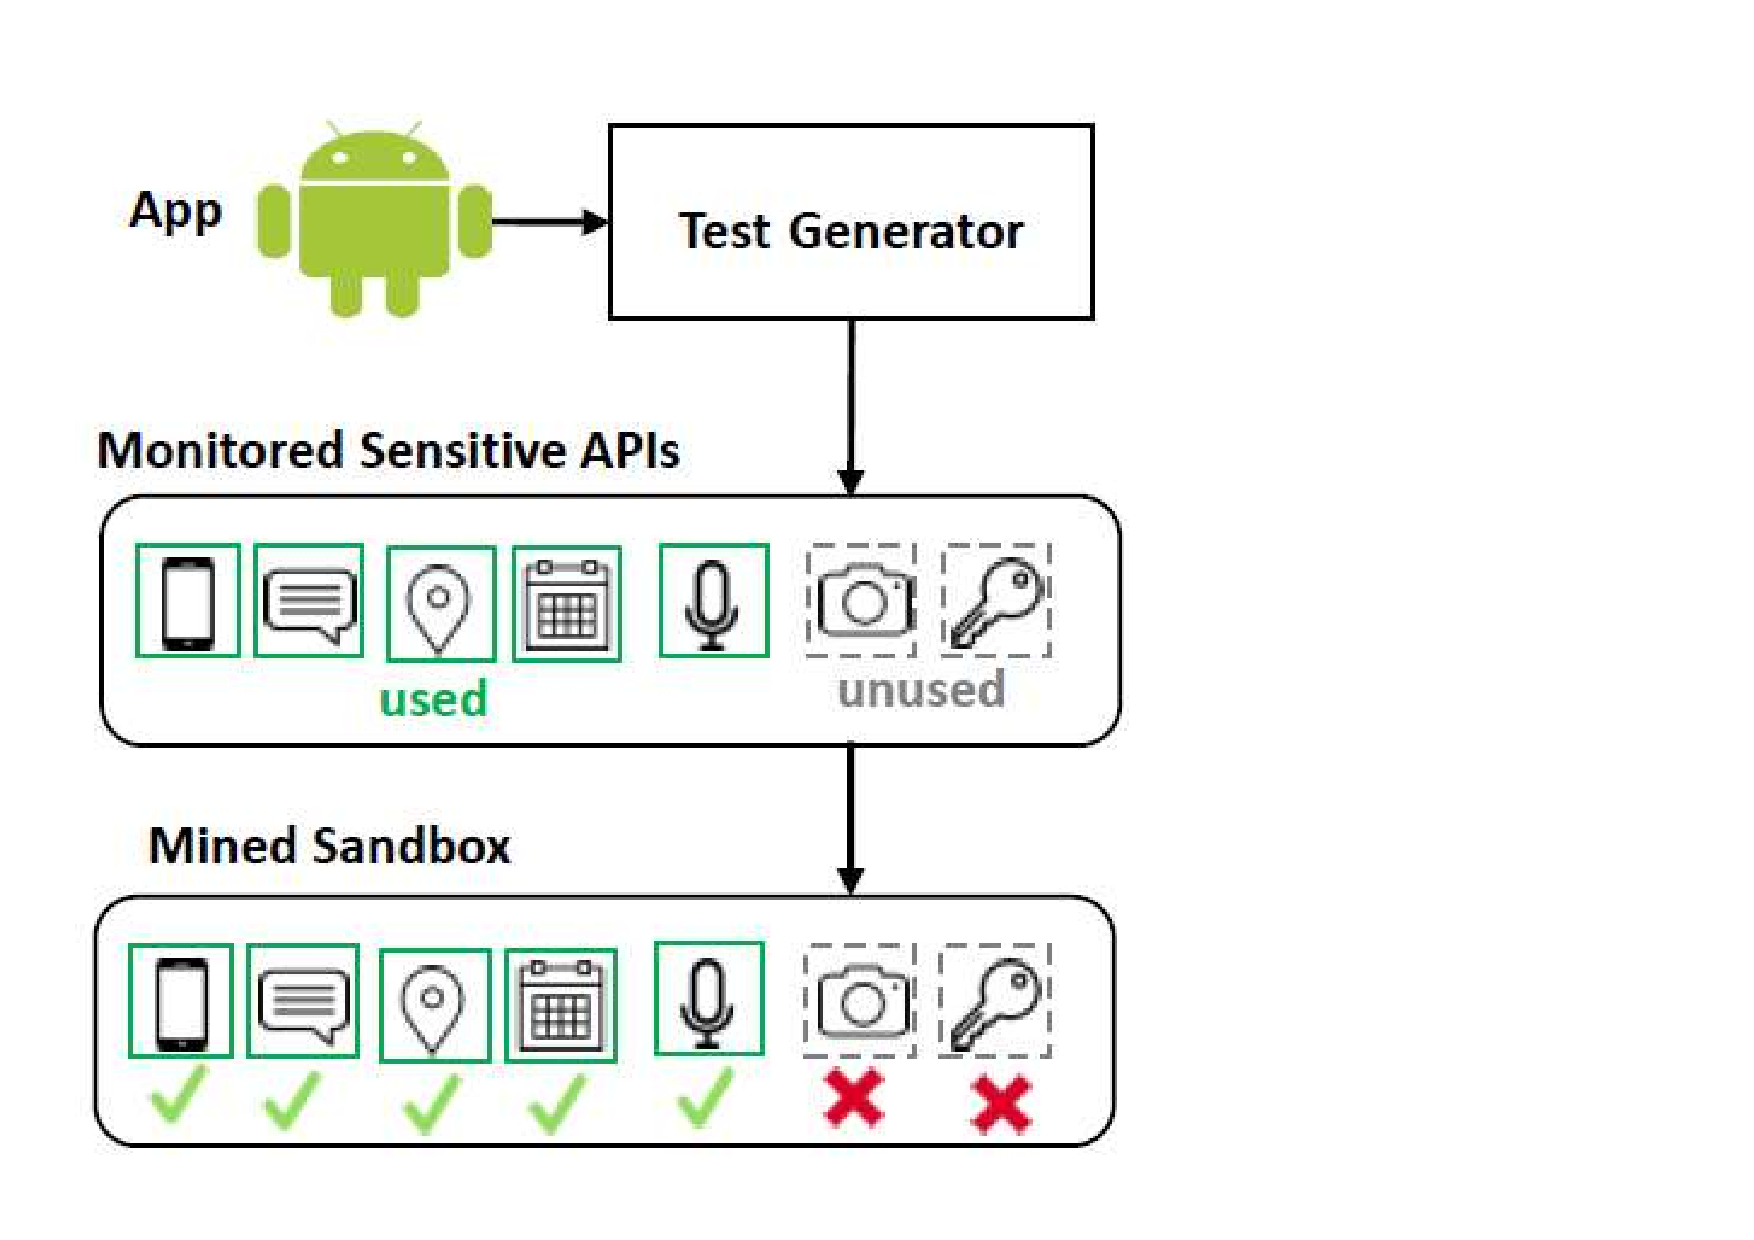
\includegraphics[scale=0.35]{images/mineSandbox.pdf}
\caption{Mine Sandbox.}
 \label{fig:mineSandbox}
\end{figure}

The Mining Android Sandbox approach~\cite{DBLP:conf/icse/JamrozikSZ16} (hereafter \mas) aims at automatically
building a sandbox through dynamic analysis (i.e., using automatic test generation tools).
The main idea is to explore apps based on their calls to sensitive APIs.
Thus, sandboxes build upon these calls to create safety rules and then block future
calls to other sensitive resources, which diverge from those found in the first exploratory
phase. Using a test generation tool named Droidmate~\cite{DBLP:conf/icse/JamrozikZ16},
Jamrozik et al.~\cite{DBLP:conf/icse/JamrozikSZ16} proposed a full fledged
implementation of the \mas, named Boxmate. 
Boxmate records the occurrences of calls to sensitive APIs and the UI events that triggers these calls,
like a button click. It is possible to configure Boxmate to record events associated with each sensitive call as
tuples (event, API), instead of recording just the set of calls to sensitive APIs. Jamrozik et al. argue that, in this way, Boxmate generates finer granularity results which
might reduce false alarms, even with the presence of reflection which is quite commonly used in
malicious apps~\cite{DBLP:conf/issta/0029BOK16}.

In fact, the \mas can be implemented using
a mix of static and dynamic analysis. In the first phase, one
can instrument an Android app to log any call to the Android sensitive methods.
After that, one can execute a test case generation tool (such as DroidBot
or Monkey) to explore the app behavior at runtime,
while the calls to sensitive APIs are recorded.
Figure~\ref{fig:mineSandbox} presents this general approach for \mas. This set of calls to sensitive APIs is then used
to configure the sandbox. 

%\todo[inline]{Since this figure is not discussed in the paper, we can remove it without any problem. I have enriched the previous paragraph, though, to make it
%  more necessary. Nonetheless, I will change this figure a bit, in order to
%represent the instrumentation phase.}



\subsection{Mining Android Sandbox for Malware Identification}

Besides being used to generate Android Sandboxes, the \mas is also effective 
to detect Android apps with suspicious behaviors~\cite{DBLP:conf/wcre/BaoLL18}. In this scenario, the \emph{effectiveness} of the approach
is estimated in terms of accuracy in which repackaged apps are identified.
The general mining sandbox approach (see Figure~\ref{fig:mineSandbox}) suggests
that the more efficient the test generator tool (for instance, in terms of code coverage),
the more accurate would be the resulting sandbox.


Figure~\ref{fig:sensitiveAPI} illustrates the \mas for
repackaged apps identification. We leverage DroidXP~\cite{DBLP:conf/scam/CostaMCMVBC20} to collect the set of sensitive APIs the versions of the apps call (benign/malign versions). As a first step, given one benign app version,
our approach first collects all calls to sensitive APIs from the app code through static analysis. Then, during the execution step,
we use dynamic analysis to collect all calls to sensitive APIs during the DroidBot test case execution. We configure DroidXP to execute DroidBot for a
period of $3$ minutes. Since some malicious app may use dynamic features (such as reflection) to introduce malicious behavior, which can change the behavior of the apps at runtime~\cite{DBLP:journals/spe/ZhangLTX18,DBLP:journals/tosem/LiTX19}, this second analysis is also important to disclose some sensitive APIs calls ignored by static analysis.

While our static analysis is made once, we execute dynamic analysis $3$ times. The result of static analysis and all executions is finally joined, forming a final set that contains all identified calls to sensitive APIs coming from the benign version of the app, as described at Figure~\ref{fig:sensitiveAPI}: ($S_{A}$, $D_{A1}$, $D_{A2}$, $D_{A3}$). We carry out the same procedure for the malicious version of the apps,
creating a distinct set of calls to sensitive APIs (now coming from the malicious version of the apps). In
a final step, we compare the two sets of calls to sensitive APIs ($Set_B, Set_M$). We use the following rules to
check for a malicious behavior. 

\begin{enumerate}
    \item If the difference between the two final sets is an empty set, we cannot distinguish the benign from the malicious version of the app (false negative).
    \item Otherwise, we successfully distinguish the benign from the malicious version of the app (true positive). 
    %\kn{Cant we replace the first part of the second point simply as "Otherwise" or is there some specific corner cases that I am missing}
\end{enumerate}

In addition, this procedure also enables us to identify the calls to sensitive APIs that are more frequently injected by the malicious version of the apps
in our dataset. 

%\fh{here I have to insert the figure}

\begin{figure}[ht]
\centering
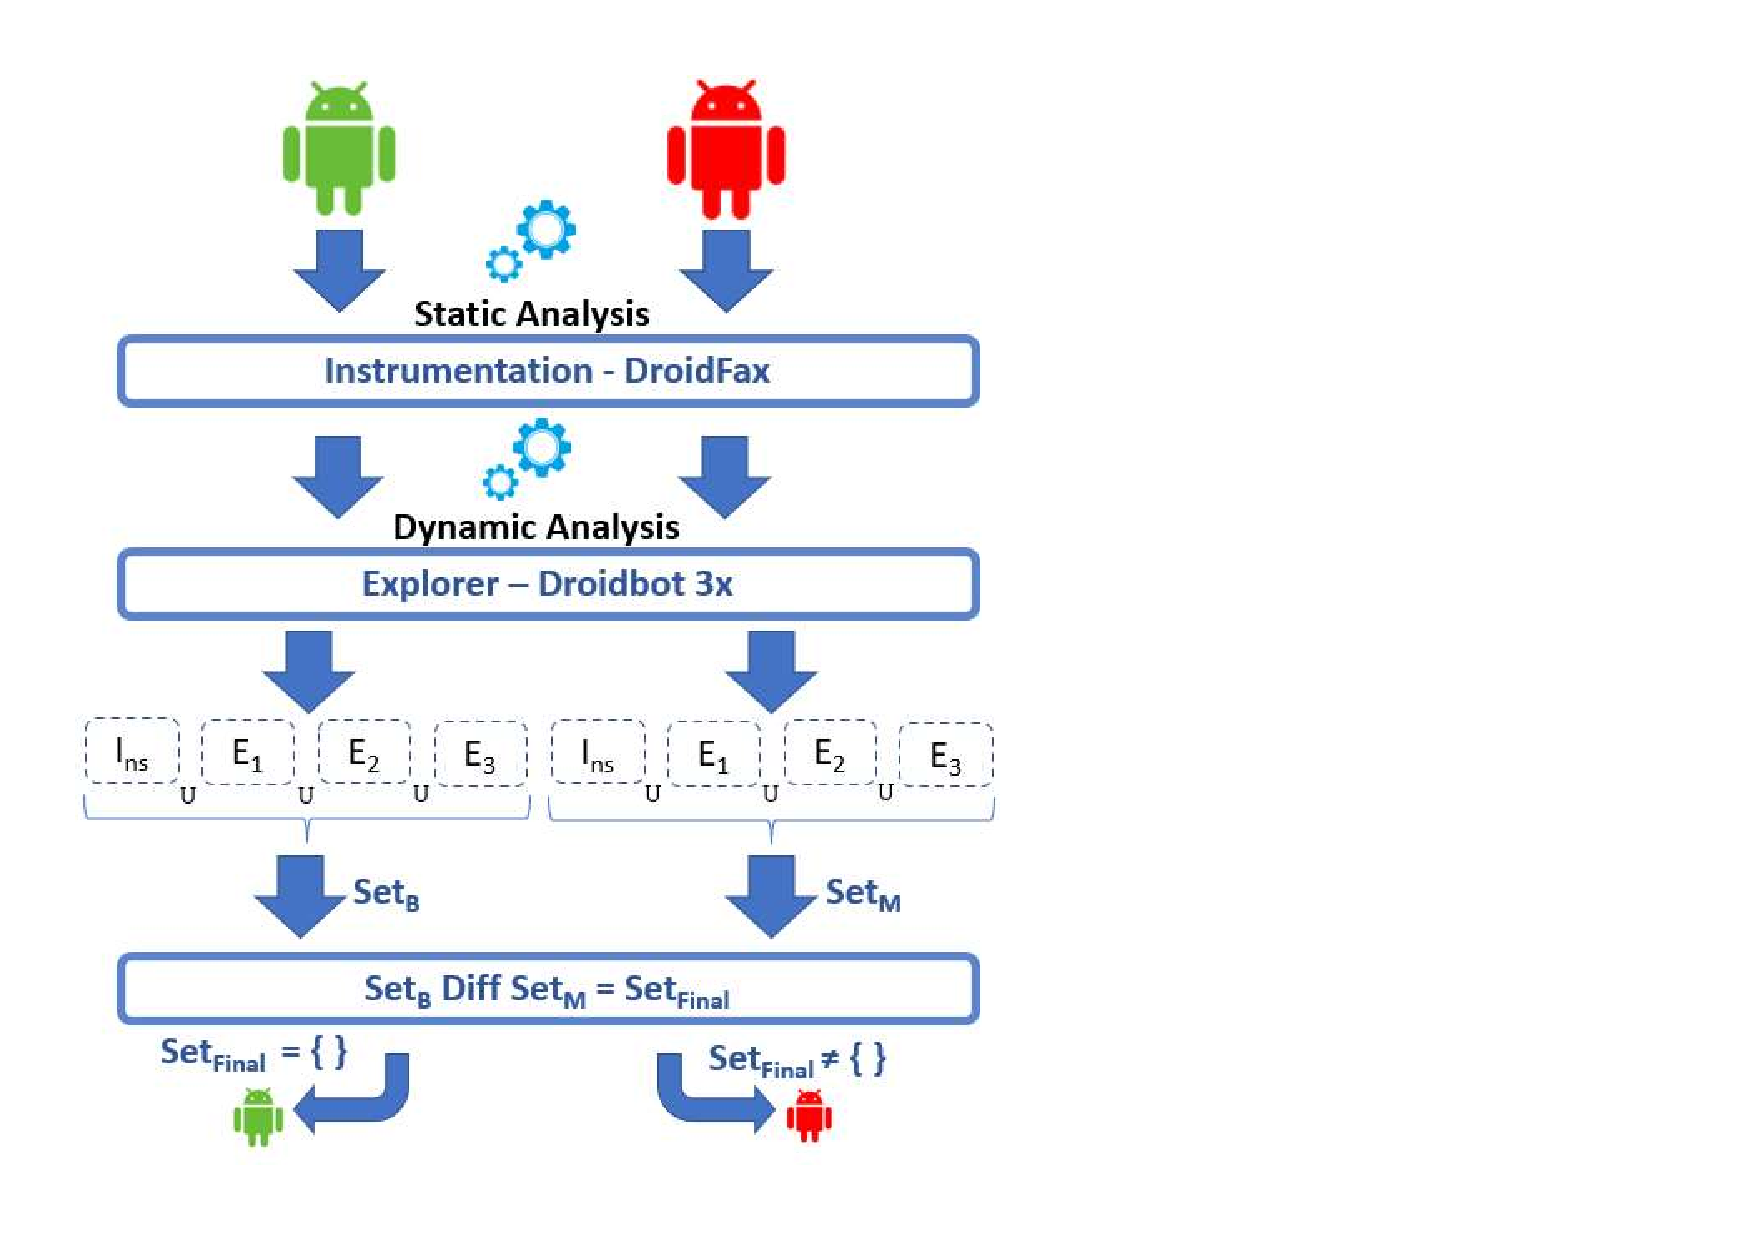
\includegraphics[scale=0.45]{images/sensitiveAPIdiff.pdf}
\caption{All procedure for suspicious app identification using sensitive API set diff.}
 \label{fig:sensitiveAPI}
\end{figure}



%\kn{I have commented out the subsection here as it seems redundant with the previous subsection}
%\subsection{The Mining Android Sandbox Approach for Malware Identification}

%The focus of our paper is in approaches that mine android sandboxes to classify Android Malware.
%There is a vast body of research in this direction. 

Costa et al. and and Bao et al.~\cite{DBLP:conf/wcre/BaoLL18,DBLP:conf/scam/CostaMCMVBC20} conducted empirical studies to investigate the effectiveness of \mas, exploring test generation tools, including DroidBot. Bao et al. found that, in general, the sandboxes constructed using test generators can detect more than $66$\% malicious apps in a dataset comprising $102$ pairs (benign/malicious). The study also presented that among $5$ test generation tools used, DroidBot~\cite{DBLP:conf/icse/LiYGC17} is the most effective sandbox.
Le et al.~\cite{le2018towards} extend the work of Bao et al. by combining more categories of sensitive APIs, and also considering the impact of actual parameters, combining sensitive APIs calls and input parameters of these APIs.
%\kn{What arguments? function parameters?}. 
Costa et al.\cite{DBLP:journals/jss/CostaMMSSBNR22} investigated the impact of static analysis to complement the accuracy of dynamic analysis tools for \mas. The study found that DroidFax~\cite{DBLP:conf/icsm/CaiR17a}, the static analysis infrastructure used in~\cite{DBLP:conf/wcre/BaoLL18}, is able to detect almost half of repackaged apps in a
dataset of $96$ pairs of benign/malicious apps.

%\todo[inline]{I could not understand why we did not cite our JSS work here}
%However, none of the aforementioned studies
% ~\cite{DBLP:conf/icse/JamrozikSZ16,DBLP:conf/wcre/BaoLL18,le2018towards}
%neither characterize the APIs included on the repackage versions nor investigate the
%possibility that trace analysis using call graph or analysis of
% the manifest file could complement the mining sandbox approach for malware identification.

\subsection{Extending the Mining Sandbox with Trace Analysis}

Our work, although closely related to previous studies, differs from them in several aspects.  First, our assessment is more comprehensive: instead of considering $102$ pairs of benign/malign apps, we execute our study considering \apps pairs of apps. Curiously, the performance of the \mas in our large dataset drops significantly. We then investigate which characteristics of the malware samples in the large dataset explain the lower performance. We observed and also explore an extension to the \mas that compare the traces from the app entry points to the calls to sensitive APIs, considering the benign and malign versions of the apps. 

As we discussed in the previous section, we build the dynamic call graphs that characterize the execution of each version of the apps in our dataset. Our goal
here is to explore how many pairs of apps call the same set of sensitive APIs, though using different call
traces. We hypothesize that differences in the traces might be used to complement the \mas for suspicious app identification. As such, here we execute the trace analysis for all app pairs of our dataset, and check if there are situations in which the basic version of the \mas was not able to correctly classify the malign version of an app as a piggybacked, however it has a different execution trace. For detecting different trace, we performed an evaluation of the dynamic call graph of each pair. Our procedure checks if there is some new node, representing a new sensitive API at malicious version, or a new edge($x$, $y$), where $x$ and $y$ indicates a method $x$ calling a sensitive method $y$.

%\rb{(Not sure if this is the right decision. I do not see any problem in running
%  this study for all pairs.)}. 
%% we  investigate those app pairs that were not described as a malware during the exploratory step, i.e,
%% the test generation tool DroidBot collected the same set of sensitive APIs for both version. If a dynamic call graph
%% of these app pairs presented different traces from entry point to sensitive APIs call at both versions, we suspect this to indicate presence of malware.
Figure~\ref{fig:callGraph} illustrates an example of benign and malicious call graphs.
At this example, although both app versions access the same set of sensitive resources, the
malicious version follows a different execution trace. 


\begin{figure}[ht]
\centering
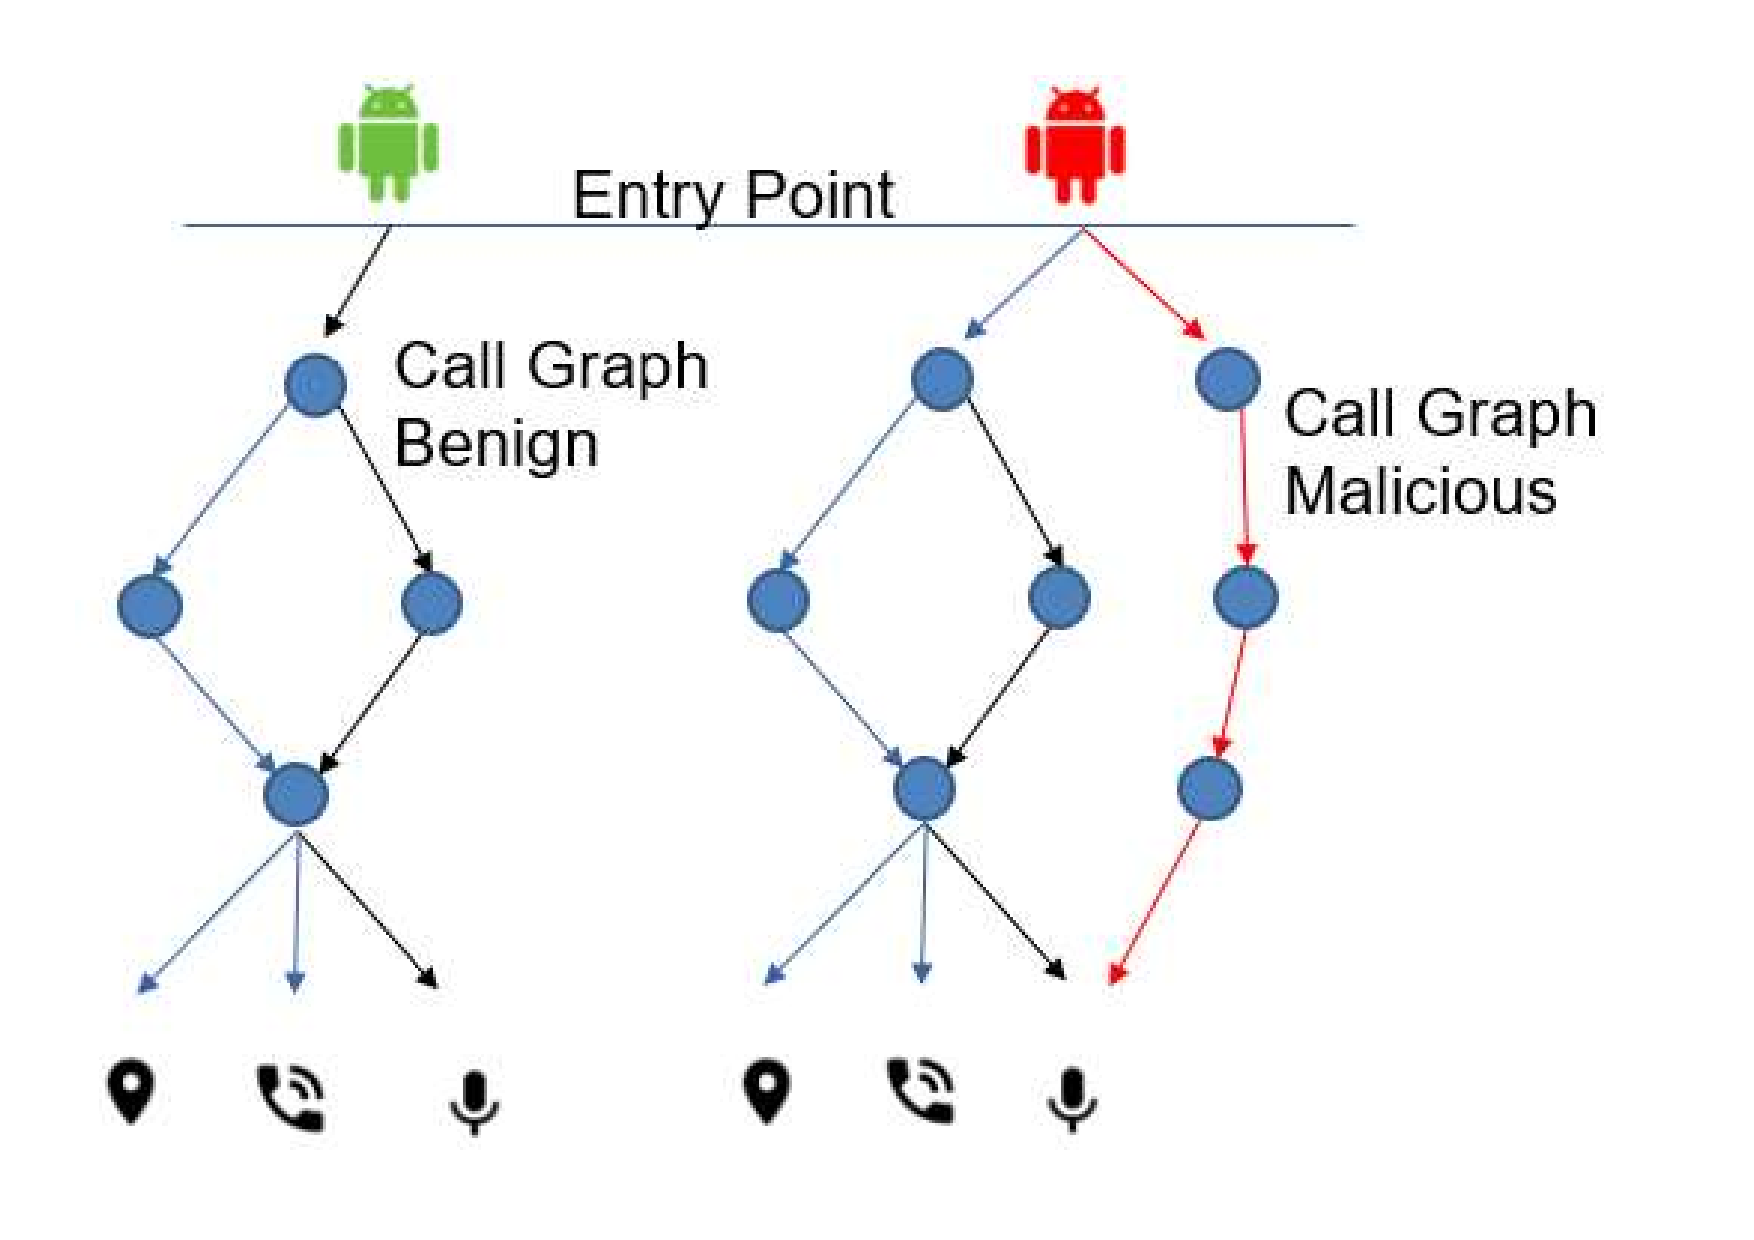
\includegraphics[scale=0.30]{images/maliciousCallGraph.pdf}
\caption{Illustrative example of the trace analysis. In this case, both versions call the same set of sensitive APIs. Nonetheless,
the traces between the entry point and the calls to sensitive APIs diverge.}
 \label{fig:callGraph}
\end{figure}


Figure~\ref{fig:maliciousTrace} shows an example of a trace injected in the malicious version of the
app \textbf{[com.android.remotecontrolppt]}. Here, the benign and malicious app versions access the same
sensitive method, \textit{getSubscriberid()}. This sensitive method returns the device's unique
subscriber ID, and requires the manifest file permission \texttt{READ\_PHONE\_STATE}, present in both app versions.
The original app accesses this method through two distinct traces (Trace 01 and Trace 02), which suggests an expected action from app user. However,
instead of the two original traces, the malicious version injected a third trace (Trace 03) containing as entry point a method that performs a stealth
computation on a background thread, \textit{doInBackground}, suggesting an action without user's awareness.


\begin{figure}
\centering
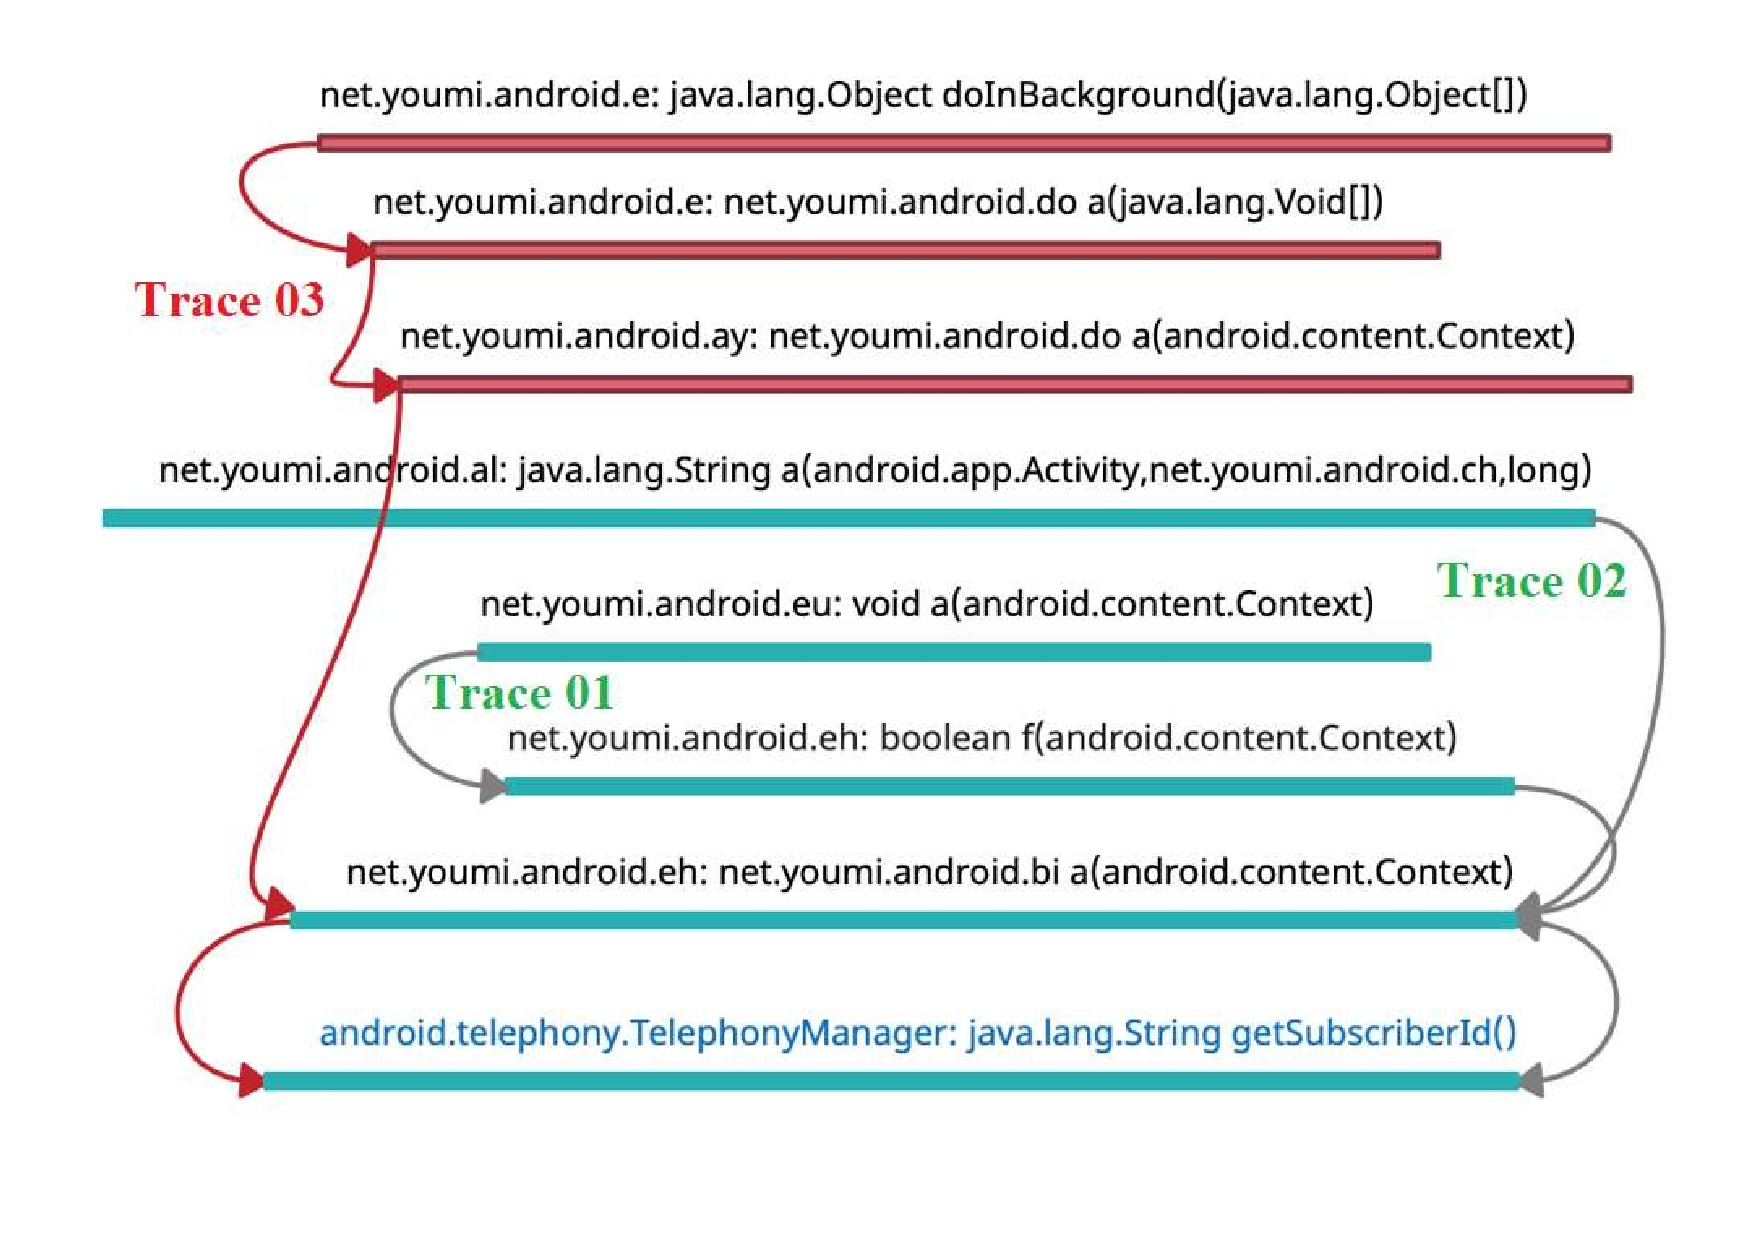
\includegraphics[scale=0.28]{images/maliciousTrace_example01.pdf}
\caption{Example of Malicious Trace.}
 \label{fig:maliciousTrace}
\end{figure}

%\section{Related Work}\label{sec:relatedwork}
In this section, we discuss prior studies in two areas: Dynamic and Static Analysis on Android and mine Sandbox.

\subsection{Dynamic and Static Analysis on Android}\label{sec:analysis}

Dynamic and Static Analysis on Android Apps are important practices for developing security apps. There is a large body of work on both analysis for Android apps security. 

Several approaches for malware detection, based on sensitive methods call and permission control Android apps~\cite{DBLP:conf/mobicom/WeiGNF12,DBLP:conf/asiajcis/WuMWLW12,DBLP:conf/sp/LiDLDG21}. Cai et al.~\cite{DBLP:journals/tse/CaiR21} presented a longitudinal study on Android apps focusing on run-time behaviors. However, this work does not explore specifically on malware detection, since only benign apps were considered in their study, and just presented possible security gaps. Fangfang et al.~\cite{DBLP:conf/wisec/ZhangHZW014} proposed ViewDroid, which models the UIs (user interface) of Android apps as a directed graph. ViewDroid identify apps repackaging, comparing graphs structures in app pairs (benign/malicious).

Through static analysis on Android Manifest files, Kim et al. proposed RomaDroid~\cite{DBLP:journals/access/KimLCP19}, a repackage Android app detector based on Manifest file. They proposed that Manifest file apps could be represented as a tree-based structure and also by a single string from this structure. Hence, RomaDroid compares the strings of the benign and malicious app, using the longest common subsequence algorithm (LCS). Au el al.~\cite{DBLP:conf/ccs/AuZHL12} also used static analysis on Android Manifest files to detect vulnerabilities in Android apps. They mapped Android APIs sensitive calls and your respective required permissions.

A relevant prior work ~\cite{DBLP:journals/tifs/0029LBKTLC17} done by Li et al. provided a systematized knowledge
on Android app security to the community. They conducted an empirical study comparing malicious repackage app with their benign counterparts (1,497 app pairs). They found that the majority of Android malware are nothing but repackaged versions of benign apps, that are done with no sophisticated way, many times automatically and using library code.

There are other works that focus on comparison of app code, and try to check similarity to detect repackaged apps. Following this approach, Crussell et al.~\cite{DBLP:conf/esorics/CrussellGC12} proposed  DNADroid, which compares program dependence graphs, and Zhou et al.~\cite{DBLP:conf/codaspy/ZhouZJN12} DroidMoss which detect and analyze repackaged apps adopting a fuzzy hashing technique.

\subsection{Mine Sandbox}\label{sec:mineSandbox}

The technique called mine sandbox consists of explores software behavior by means of automatic test generation tools and, thus, prevent
Android apps from suspicious behaviors. Using a test generation tool named Droidmate~\cite{DBLP:conf/icse/JamrozikZ16}, Jamrozik et al.~\cite{DBLP:conf/icse/JamrozikSZ16} proposed an approach called Boxmate, the first mine Sandbox approach for Android environment. Boxmate records the occurrences of calls to sensitive APIs and input parameters. They found that Boxmate has low false alarm rate when checking Boxmate against 18 benign app that uses reflection API (\textit{java.util.reflect}) package. The reflection API at runtime can modify behavior of classes, interfaces and methods, and it is quite commonly used at malicious app~\cite{DBLP:conf/issta/0029BOK16}. Jamrozik et al. did not consider real malware to validate their approach, beyond they used a small sample of Android apps.

Bao et al.~\cite{DBLP:conf/wcre/BaoLL18} conducted an empirical study to investigate the effectiveness of mine sandboxes, exploring test generation tools, including Droidmate. The authors found that in general, the sandboxes constructed by test generator tools can detect more than $70$\% malicious apps in a dataset comprising $102$ pairs (benign/malicious). The study also presented that among 5 test generate tools used, DroidBot~\cite{DBLP:conf/icse/LiYGC17} constructed the sandbox more efficient to detect malware.

However, Bao et al. do not investigate the effectiveness of mine sandboxes considering parameter values in the called APIs to compose the sandbox. To mitigate this issue, Le et al.~\cite{le2018towards} extend the previous work, combining more categories of APIs, and now considering parameters.

Neither of the studies in ~\cite{DBLP:conf/icse/JamrozikSZ16} and ~\cite{DBLP:conf/wcre/BaoLL18}~\cite{le2018towards} investigated the possibility of Path Analysis using call Graph complements mine sandbox technique, in terms of malware detection. They also do not considered the possibility of a static analysis on Manifest file apps, complement mine sandbox at same objective. Hence, our work although closely to aforementioned studies, differs from them in three aspects: First, these approaches used a little sample of app pairs. To improve the study, we conducted our work exploring $824$ pair apps and also included another test generator tool for Android, did not used at Bao et al. study, Humanoid~\cite{DBLP:conf/kbse/LiY0C19}---actually a DroidBot evolution. Second, we explore dynamic call graphs, exploring traces of apps version (benign/malicious) from entry point to sensitive API access, adding information about call graphs at our study. Third, we also consider explore suspicious features extract from Manifest file apps.
%\section{Sandbox Solution and its Weakness}\label{sec:sandbox}
\section{Experimental Setup}\label{sec:experimentalSetup}

The goal of this research is to build an in-depth understanding about
the performance of the \mas for detecting malware. To this
end, we conduct our research using a dataset of repackaged apps one order of magnitude
larger than previous studies~\cite{DBLP:conf/wcre/BaoLL18,DBLP:journals/jss/CostaMMSSBNR22}. Altogether,
explore the the following research questions:

\begin{enumerate}[(RQ1)]
\item \rqa
\item \rqc
\item \rqd
\textcolor{blue}{\item \rqe}
\end{enumerate}

In this section, we describe our study settings. First, we present how we mined the samples of Android apps that we
use as a dataset for our study (Section~\ref{sec:dataset}).  Then, we describe the data
collection and data analysis procedures (Sections~\ref{sec:dataCollectionProc} and~\ref{sec:dataAnalysisProc}). Finally,
we detail our experiment configuration on Section~\ref{sec:hardware}. 


\subsection{Malware Dataset}\label{sec:dataset}


%Our experiment aims to compute if an app pair from a given sample is a malware variant of its corresponding original app.
To investigate our research questions, we shall run our infrastructure on a representative dataset and
estimate the \mas performance (in terms of accuracy). Our dataset shall also
be \textit{labeled}, i.e., the interest characteristic of each app, like similarity and malware family, should be known beforehand. 

\subsubsection{Procedures for Building the Dataset}

Figure~\ref{fig:dataset} presents the methodology we use to extract the dataset for our study. We start with an original dataset containing 15,297
pairs of original/repackaged Android apps, \textcolor{blue}{with 2,776 original apps. Many original apps are repackaged several times by different attackers, with a minimal, and maximum times of 1 and 176, respectively}~\cite{DBLP:journals/tse/LiBK21}. This original dataset
has been curated using automatic procedures that mine repackaged apps from the well-known Androzoo repository~\cite{DBLP:conf/msr/AllixBKT16}. However, among these 15,297 app pairs, we fail to execute our study in 1,176 original apps. We could not either instrument some of them using DroidFax~\cite{DBLP:conf/icsm/CaiR17a} or we fail to install some of them on the emulator---due to compatibility issues with the Android SDK. After removing \textcolor{blue}{incompatible original apps}, we were left with \textcolor{blue}{3,827 samples of app pairs}. To build our final dataset (hereafter \cds), we queried the \vt repository to find out which original version of the apps have been labeled as a malware. We exclude these samples from our dataset---since the \mas assumes that the original version of an app is legitimate. \vt is a well-known mechanism for scanning software assets (such as Android apps) using more than 60 anti-virus
engines~\cite{DBLP:journals/ese/KhanmohammadiEH19}. In the end, we are left with our \cds of \apps apps which we use for this study.
In our research, we also consider a small dataset (hereafter \sds) used in previous studies~\cite{DBLP:conf/wcre/BaoLL18,DBLP:journals/jss/CostaMMSSBNR22}.

 \begin{figure}[htb]
  \includegraphics[width=\columnwidth]{images/dataset.pdf}
  \caption{Malware samples in the Complete Datasets.}
  \label{fig:dataset}
\end{figure}



%starting from an initial sample of 3344 repackaged pairs of apps available in AndroZoo~\cite{DBLP:conf/msr/AllixBKT16}.
%We do not use any particular criteria for selecting the initial sample.
%Nonetheless, due to compatibility issues we found---either during the instrumentation phase (using DroidFax) or during the execution
%phase using the Android emulator---we end-up with our final dataset (hereafter \cds) that contains \apps pairs of
%repackaged apps (36\% of the initial subset repackaged apps).
%\fh{At this paragraph I change the term set to Subset since 3344 is a subset of 15.000 repackage pair}

%\kn{This whole part about Virustotal needs a bit more elaboration. Ideally, including a citation explaining why we go for this additional method of classifying whether something as a malware or not. Since we already start with the app pairs, we sort of already know the malicious and benign version right? }

\subsubsection{Features of the Datasets}
 
We queried the \vt repository to find out which repackaged apps in our
dataset have been indeed labeled as a malware.
%, and we took this decision since the output of \vt can change over time~\cite{vt-label}.\fh{Here I inserted a litle discription of
% VT and inserted some reference}
%(\kn{two out of how many antiviruses are included by Virustotal}). 
According to \vt, in the \sds (102 pairs),
69 of the repackaged apps (67.64\%) have been identified as a malware by at least two
\ses. Here we only consider that a repackaged version of an app is a malware if \vt reports that at least
two \ses identify a malicious behavior within the asset. This is in accordance with previous research~\cite{vt-label,DBLP:journals/ese/KhanmohammadiEH19}. Conversely, considering the \cds, at least two security engines identified \malwares out of the \apps repackaged apps as malware (\malwaresP\%).

Classifying malware into different categories is a common practice. For instance, Android malware can be classified into categories
like riskware, trojan, adware, etc. Each category might be further specialized in several malware families, depending of its
characteristics and atack strategy---e.g., steal network info (IP, DNS, WiFi), collect phone info,
collect user contacts, send/receive SMS, and so on~\cite{DBLP:conf/iccns/RahaliLKTGM20}.
According to the
\avt~\cite{avclass2-paper}, the malware samples in the \sds come from $17$ different families---most of them from the Kuguo (49.27\%) and Dowgin (17.39\%) families.  
Our \cds, besides a large sample of repackaged apps (\apps in total),
comprises \textcolor{blue}{52} families of malware we collected using the \avt---most
of them from the Gappusin \textcolor{blue}{(40.17\%)} family.

We also characterize our dataset according to the similarity
between the original and repackaged versions of the apps, using the  
SimiDroid tool~\cite{DBLP:conf/trustcom/0029BK17}. SimiDroid quantifies the similarity
based on (a) the methods that are either identical or similar in both versions of the apps (original and repackaged versions),
(b) methods that only appear in the repackaged version of the apps (new methods), and (c) methods that only appear in the
original version of the apps (deleted methods).
Our \cds has an average similarity score of \textcolor{blue}{92.72\%}---with the follow distribution \textcolor{blue}{(84 of
app pairs have a similarity score of less than 25\%, 48 of app pairs
between 25\% and 50\%,  62 of the apps between 50\% and 75\%,
and 3017 of the apps with more than 75\%). The \sds presents a lowest
similarity index average (89.41\%). }


After executing our experiments, we identified the  most frequently abused sensitive APIs called by the repackaged version of our samples.
We observed that upon execution of all samples from the \cds, malicious app versions injected \textcolor{blue}{$126$} methods from sensitive APIs (according to the
AppGuard~\cite{DBLP:conf/esorics/BackesGHMS13} security framework). Malicious code may use these APIs to compromise system security and
share sensitive data. Table~\ref{tab:APIused} presents a list of methods from sensitive APIs the  malicious versions of the apps
frequently inject.

\begin{table*}[ht]
  \caption{Sensitive APIs that frequently appear in the repackaged versions of the apps. The
    \emph{Occurrences} column gives the number of distinct repackaged apps that introduce a call
  to a sensitive method.}
\centering
  \begin{tabular}{lc}

    \hline
    Method of Sensitive API & Occurrences \\
    \hline \\
    android.telephony.TelephonyManager: java.lang.String getNetworkOperatorName() &  193\\
    android.content.ContentResolver: android.database.Cursor query(android.net.Uri,java.lang.String[],...,...) &  185 \\
    android.database.sqlite.SQLiteOpenHelper: android.database.sqlite.SQLiteDatabase getWritableDatabase() &  170 \\
    java.lang.reflect.Field: java.lang.Object get(java.lang.Object) &  170 \\
    android.database.sqlite.SQLiteDatabase: android.database.Cursor query(java.lang.String,java.lang.String[],...,...,...,...,...) &  168 \\
    android.telephony.TelephonyManager: int getPhoneType() &  164\\
    java.lang.reflect.Field: int getInt(java.lang.Object) &  156\\
    android.database.sqlite.SQLiteOpenHelper: android.database.sqlite.SQLiteDatabase getReadableDatabase() &  154\\
%    android.telephony.TelephonyManager: java.lang.String getNetworkOperatorName() &  123 \\
\\\hline
\end{tabular}
\label{tab:APIused}
\end{table*}

%%  \end{tabular}
%%  %\end{small}
%%  \label{tab:APIused}
%% \end{table*}
%\end{landscape}








It is important to highlight that our sample comes
from different Android app stores. Most of our repackage apps come from a non-official
Android app store, Anzhi~\cite{anzhi}. However, some repackaged apps also come from the
official Android app store, Google Play.


%\begin{figure}[ht]
%\centering
%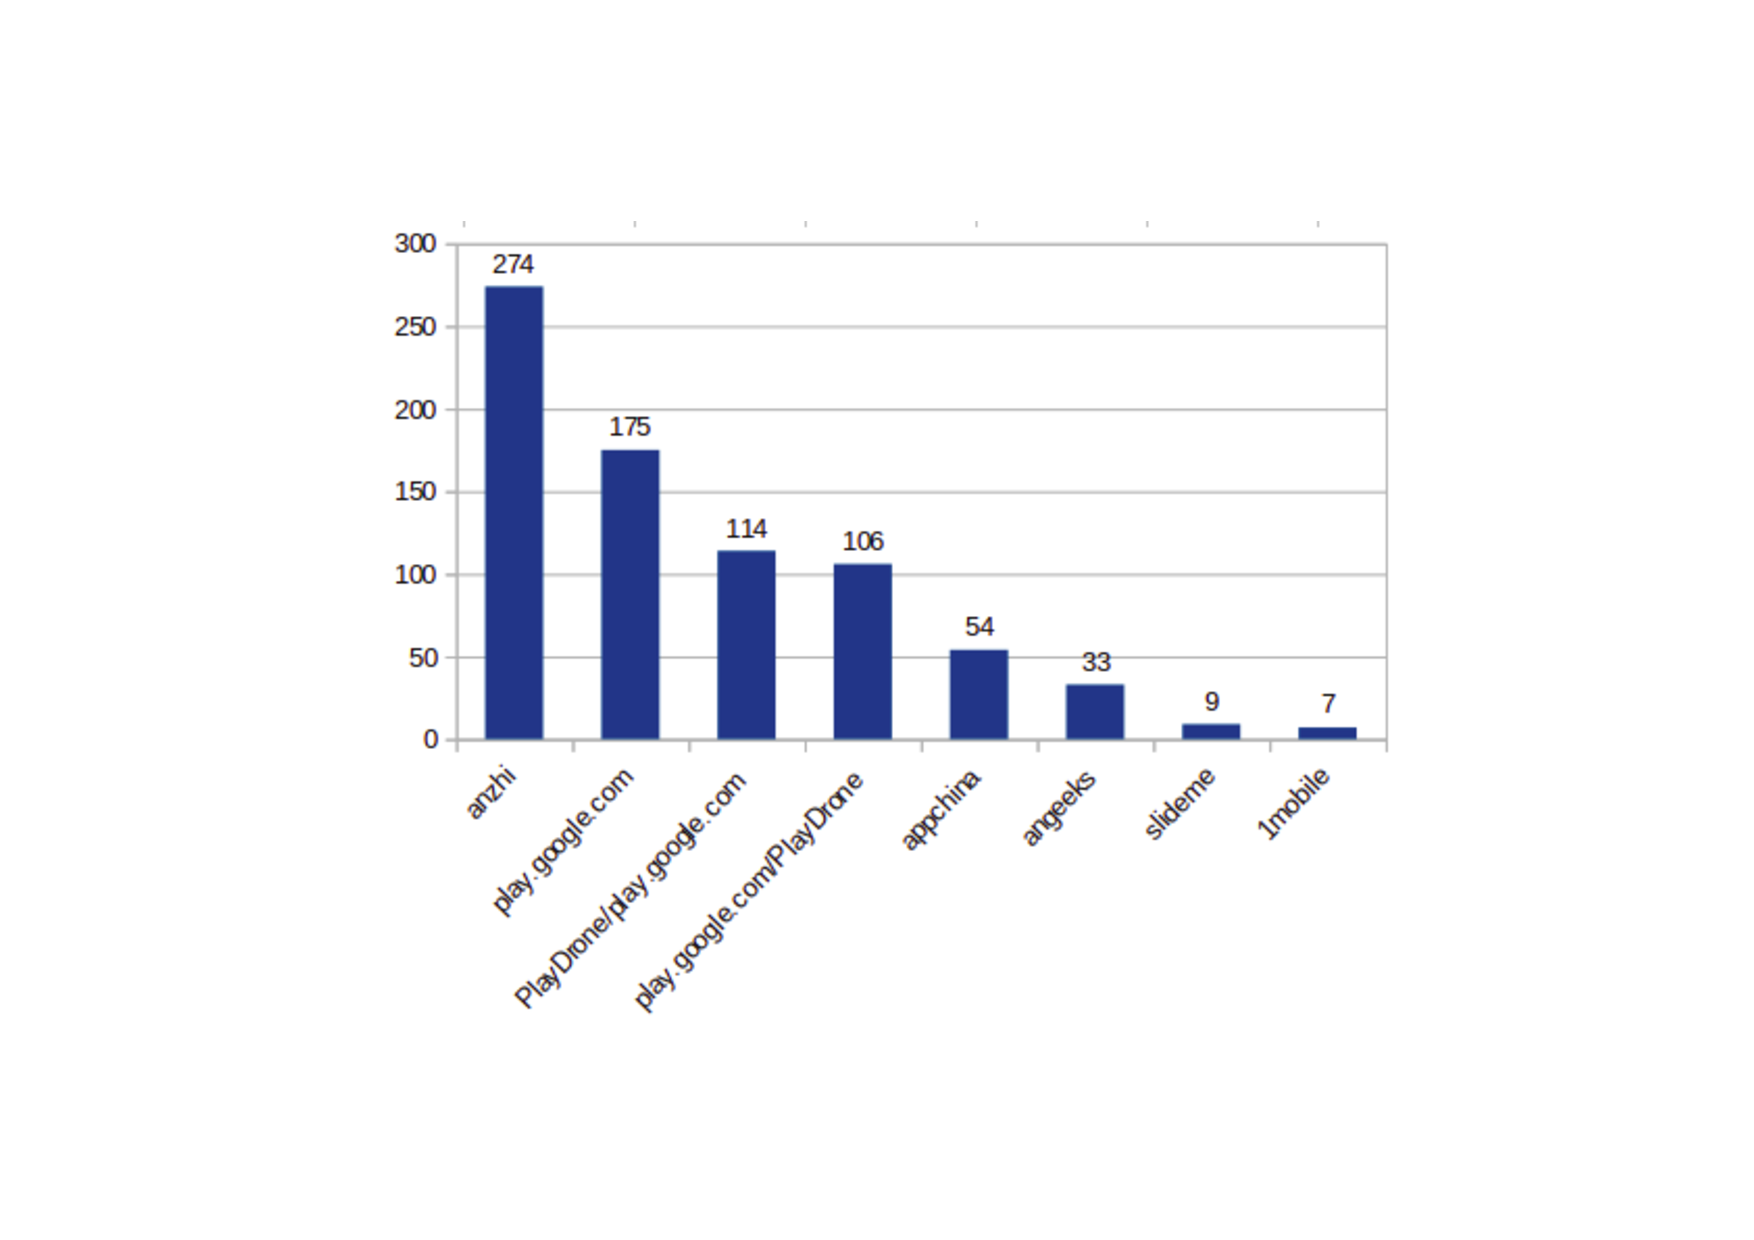
\includegraphics[scale=0.43]{images/stores.pdf}
%\caption{Markets where malware was discovered.}
% \label{fig:stores}
%\end{figure}


\subsection{Data Collection Procedures} \label{sec:dataCollectionProc}

We take advantage of the DroidXP infrastructure~\cite{DBLP:conf/scam/CostaMCMVBC20}
for data collection. DroidXP allows researchers to compare 
test case generation tools in terms of malicious app behaviors identification, using the \mas. Although the comparison of test
case generation tools is not the goal of this paper, DroidXP
was still useful for automating the following steps of our study.


\begin{enumerate}[S1]
 \item \textbf{Instrumentation}: In the first step,
we configure DroidXP to instrument all pairs of apps in our dataset.
Here, we instrument both versions of the apps (as APK files) to collect relevant information during their execution. Under the hood, DroidXP leverages
DroidFax~\cite{DBLP:conf/icsm/CaiR17a} to instrument the apps and collect static
information about them. To improve the performance across multiple executions,
this phase executes only once for each version of the apps in our dataset.

\item \textbf{Execution}: In this step, DroidXP first installs the (instrumented) version of the APK files in the Android emulator we use in our experiment (API 28) and then starts a test case generation tool for executing both app versions (original and repackage). We execute the apps via DroidBot~\cite{DBLP:conf/icse/LiYGC17}, mostly because previous research works report the best accuracy of the sandboxes built using the \mas and the DroidBot as test case generation tool. To also ensure that each execution gets the benefit of running on a fresh Android instance without biases that could stem out of history, DroidXP wipes out all data stored on the emulator that has been collected from previous executions.


\item \textbf{Data Collection}: During the execution of the instrumented apps, we collect all relevant information (such as calls to sensitive APIs, test coverage metrics, and so on). We use this information to analyse the performance of the \mas for detecting malicious behavior.
\end{enumerate}

\subsection{Data Analysis Procedures} \label{sec:dataAnalysisProc}



We consider that a test
generation tool, in our case, DroidBot, builds a sandbox that labels a repackaged version
of an app as a malware if there is at least one call to a sensitive APIs that (a) was observed
while executing the repackaged version of the app and that (b) was not observed while
executing the original version of the same app. If the set of sensitive methods that only the repackaged version of an app calls is empty,
we conclude that the sandbox does not label the repackaged version of an app as a malware. The set of sensitive APIs used at our work was defined in the AppGuard framework~\cite{DBLP:conf/esorics/BackesGHMS13}, which was based on the mapping from sensitive APIs to permissions proposed by Song et al.~\cite{DBLP:conf/ccs/FeltCHSW11}. We triangulate
this information with the outputs of \vt, which might lead to one of the following
situations:

\begin{itemize}
\item {\bf True Positive (TP)}. The \mas labels a repackaged version as a malware and, according to
  \vt, at least two \ses label the asset as a malware.
  
\item {\bf True Negative (TN)}. The \mas does not label a repackaged version as a malware and,
  according to \vt, at most one \se labels the asset as a malware. 

\item {\bf False Positive (FP)}. The \mas labels a repackaged version as a malware and, according to
  \vt, at most one \se labels the asset as a malware.

\item {\bf False Negative (FN)}. The \mas does not label a repackaged version as a malware, and
  according to \vt, at least two \ses label the asset as a malware.
\end{itemize}

We compute \emph{Precision}, \emph{Recall}, and \emph{F-measure} ($F_1$) from
the number of true-positives, false-positives, and false-negatives (using standard
formulae). We use basic statistics (average, median, standard deviation) to identify the
accuracy of the \mas for malware classification, in both
datasets we use in our research---i.e., the \sds
with 102 pairs of apps and our \cds with
\apps pairs. We use the Spearman Correlation~\cite{spearman-correlation} method and
Logistic Regression~\cite{statistical-learning} to understand the strengths of
the associations between the similarity index between the original and the repackaged versions
of a malware with the \mas accuracy---that is,
if the approach was able to correctly classify an asset as malware. We also use existing tools to reverse engineer a sample of repackaged
apps in order to better understand (the lack of) accuracy
of the \mas.



%\fh{I removed the item C of this section that talk about hardware and execution time.}

\subsection{Environment Configuration}\label{sec:hardware}

%\todo[inline]{RB: later, if we need space, we can safely comment this section out.}

We deployed our experiment on a 32-Core, AMD EPYC 7542 CPU, 512 GB RAM, storage Samsung SSD 970 EVO 1TB machine running a 64-bit Debian GNU/Linux 11. We also configured our emulator to run all selected apps on Google Android version 9.0, API 28, 512M SD Card, 7GB internal storage, with X86 ABI image.
For our study, we configured DroidXP to run each of the \apps app pairs using DroidBot for 3 minutes. To mitigate noise, we repeated the full process 3 times,  which took around \textcolor{blue}{$965$} machine hours in total. Although it was possible to run more than 10 emulators in parallel on one physical machine, to avoid any interference resulting from context switching within the operating system, we chose to run one emulator at a time. Hence, all processes took around 45 days, 40 days for experiment execution and additional 5 days for environment configuration.


\section{Results}\label{sec:results}


In this section, we detail the findings of our study.  We remind the reader that our main goal with this study is to
better understand the strengths and limitations of the \mas for malware detection using the state-of-the-art
test case generation tool (DroidBot). We explore
the results of our research in two datasets: the \sds (102 pairs of apps) and the
\cds (\apps pairs of apps).


\subsection{Exploratory Data Analysis of Accuracy}


{\bf \sds.}
After running the dynamic analysis via DroidBot, our infrastructure produces
a dataset with the sensitive methods that both app versions call during their execution. We consider that a test
generation tool, in our case, DroidBot, builds a sandbox that labels a repackaged version
of an app as a malware if there is at least one call to a sensitive method that (a) was observed
while executing the repackaged version of the app and that (b) was not observed while
executing the original version of the same app. 
If the set of sensitive methods that only the repackaged version of an app calls is empty,
we conclude that the sandbox does not label the repackaged version the app as a malware. We triangulate
this information with the outputs of \vt, which might lead to one of the following
situations:

\begin{itemize}
\item {\bf True Positive}. The \mas labels a repackaged version as a malware and, according to
  \vt, at least two \ses label the asset as a malware.
  
\item {\bf True Negative}. The \mas does not label a repackaged version as a malware and,
  according to \vt, at most one \se labels the asset as a malware. 

\item {\bf False Positive}. The \mas labels a repackaged version as a malware and, according to
  \vt, at most one \se labels the asset as a malware.

\item {\bf False Negative}. The \mas does not label a repackaged version as a malware, and
  according to \vt, at least two \ses label the asset as a malware.
\end{itemize}



Considering the \sds (102 apps), the \mas for malware detection 
classifies a total of 69 repackaged versions as malware (67.64\%).
This result is close to what Bao et al. report. That is, in their
original paper,  the \mas approach using DroidBot classifies 66.66\% of the
repackaged version of the apps as malware~\cite{DBLP:conf/wcre/BaoLL18}.
This result confirms that we were able to reproduce
the findings of the original study using our
infrastructure. 

\tb{1}{We were able to reproduce the results of
  existing research using our infrastructure,
  achieving a malware classification in the
  \sds close to what has been reported in
  previous studies.}

In the previous studies~\cite{DBLP:conf/wcre/BaoLL18,DBLP:journals/jss/CostaMMSSBNR22},
the authors assume that all repackaged versions contain a
malicious behavior. For this reason, the authors do not
explore accuracy metrics such as Precision, Recall, and
F-measure ($F_1$). As we mentioned, in this paper we take advantage
of \vt to label our dataset and build a ground truth: we only
consider a repackaged version of an app a malware if the results
of our \vt query report that at least two
\ses identify a malicious behavior in the asset.
The first row of Table~\ref{tab:accuracy} shows that the
vanilla \mas achieves an accuracy of 0.89. 

\begin{table*}[htb]
  \caption{Accuracy of the \mas in both datasets.}
\centering{
  \begin{tabular}{llrrrrrr} \toprule
    Approach       & Dataset & TP   & FP  & FN  & Precision & Recall & $F_1$ \\ \midrule
    Vanilla \mas   & \sds    & 62   & 7   & 7   & 0.89      & 0.89   & 0.89  \\
    \mas + Traces  & \sds    & 67   & 18  & 2   & 0.78      & 0.97   & 0.87  \\
    Vanilla \mas   & \cds    & 173  & 173 & 286 & 0.5       & 0.37   & 0.42  \\
    \mas + Traces  & \cds    & 214  & 326 & 245 & 0.39      & 0.46   & 0.42  \\ \bottomrule
  \end{tabular}
  }
  \label{tab:accuracy}
\end{table*}

We also investigate if one could improve the performance of
the \mas using a more elaborated comparison approach.
That is, instead of only comparing the sets of calls to sensitive APIs,
here we also compare the traces from entry points to such a calls. If there is
at least one trace that appears only during the execution of the
test cases in the repackaged version of the app, we
label that version as a malware.

As we already discussed in this section, the vanilla \mas fails
to detect seven malware on the \sds (FN column, first row of Table~\ref{tab:accuracy}),
using DroidBot as a test case generator tool. Introducing trace analysis reduces the
number of false negatives to two, with the side effect of increasing the
number of false positives from 7 to 18 (see the second row of Table~\ref{tab:accuracy}).
In general, the accuracy ($F_1$) of the \mas using trace analysis drops from 0.89 to 0.67.


\tb{2}{Although the use of Trace Analysis reduces the number of
  false negatives (in comparison with the vanilla \mas), it slightly decreases the
  overall accuracy ($F_1$) of the \mas to detect malware,
  from 0.89\% to 0.87\% in the \sds.} 



{\bf \cds.} Surprisingly, when applied to our complete dataset (\apps apps), the \mas
labels a total of 346 repackaged apps as malware (28.76\% of the total number of repackaged
apps)---for which the repackaged version calls at least one additional sensitive API.
Our analysis also reveals a {\bf negative result} related to the accuracy of the approach: here,
the accuracy is much lower in comparison to what we reported for the
\sds (see the third row of Table~\ref{tab:accuracy}), dropping from 0.89 to 0.42 (a reduction of 47.19\% in terms of $F_1$).
This result indicates that, when considering a more representative dataset, the accuracy of the \mas using
DroidBot drops significantly. 


\tb{3}{
  The \mas for malware detection
  leads to a substantially lower performance on the
  \cds (1204 pairs of apps),
  dropping the accuracy in 47.19\% smaller in comparison to
  what we observed in the \sds.}


Therefore, the resulting sandbox we generate using
DroidBot suffers from a significantly low accuracy rate when considering a large and more representative dataset, 
which encouraged us to endorse efforts aimed at identifying potential blindspots with such approaches.
Nonetheless, enriching the \mas with trace analysis also
decreases the overall accuracy in the \cds (even though we reduce the
number of false negatives with trace analysis, the increasing in the
number of false positives negatively impacts the performance of the
approach). This is shown in the fourth row of Table~\ref{tab:accuracy}.

\todo[inline]{The previous paragraph now seems a bit unnecessary.}

\subsection{Assessment Based on \sscore}

Figure~\ref{fig:ss} shows the \sscore distribution
over the two datasets we use in our research
(the small and the complete datasets).
Recall that the \sscore measures how similar the
benign and malicious versions of an app are.
The average \sscore of the
\sds is 0.77 (median of 0.86 and sd of 0.22). Contrasting,
the average \sscore of the complete dataset is
0.62 (median of 0.72 and sd of 0.32).

\begin{figure}
  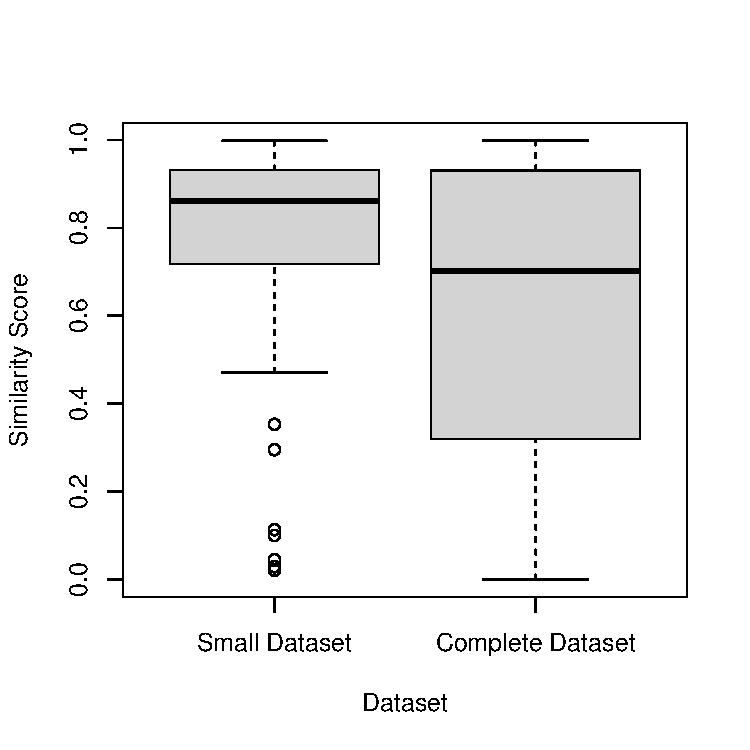
\includegraphics[width=\columnwidth]{images/similarity-1.pdf}
  \caption{\sscore of the malware samples in the small and complete datasets.}
  \label{fig:ss}
\end{figure}

Here we hypothesize that \sscore could explain
the differences of \mas we observed
when comparing the accuracy results for both
datasets. We first use Logistic Regression to test this hypothesis,
assessing the strength of the association between label correctness and
the \sscore. The logistic regression results reveal
a negative and real association ($p$-value $<$ 0.0005). This find suggests
that the \mas is more likely to assign a correct label to
a repackaged app in the cases where its \sscore with the original
app is small. This is a an unexpected result, since
we found a higher accuracy on the \sds even though
it presents a higher \sscore on average, in comparison with the \cds. 

In a further analysis, we use the \emph{K-Means} algorithm to split the
\cds into five clusters, according to the \sscore. We then
estimate the accuracy for each cluster, as
we show in Table~\ref{tab:ss-clusters}. Note that the \mas
achieves a percentage of hits close to 70\% in the clusters 1~--~4, that present an average \sscore of at most 0.76.


\tb{4}{There is a negative and real association between
  the \sscore and the \mas performance. Nonetheless,
  the \sscore does not explain the lower
accuracy of the \mas in the \cds.}

\begin{table}[ht]
  \caption{Characteristics of the clusters. Note that the percentage of
    hits decreases in the cluster with the higher average \sscore.}
 \centering
 \begin{tabular}{rrrrr}   \toprule
   cId & Total of Samples & Total of Hits & (\%) of Hits & \sscore \\ \midrule
   1 & 196 & 134 & 68.37 & 0.07 \\ 
   2 & 146 & 101 & 69.18 & 0.29 \\ 
   3 & 182 & 131 & 71.98 & 0.54 \\ 
   4 & 247 & 175 & 70.85 & 0.76 \\ 
   5 & 431 & 202 & 46.87 & 0.94 \\ \bottomrule
 \end{tabular}
 \label{tab:ss-clusters}
 \end{table}


\subsection{Assessment Based on Malware Family}

The similarity assessment we discussed in the previous
section does not explain the low performance of the
\mas on the \cds. Recall that the \cds is more heterogeneous
both in terms of similarity and malware families. So,
we hypothesize that the families of the malwares in the \cds could
better explain the poor performance of the \mas on the \cds.
Indeed, in the \cds, we identified a total of
57 families of malwares, though the most frequent
ones are \gps (198 samples),
\emph{kuguo} (44 samples), \emph{revmob} (36 samples),
and \emph{dowgin} (33 samples). Together, they
account for 67.75\% of the repackaged apps in our
complete dataset labeled as malware according to \vt.

This family distribution in the \cds is
significantly different from the family
distribution in the \sds---where the
families \emph{kuguo} (34 samples), \emph{dowgin} (12 samples),
and \emph{youmi} (5 samples) account for
73.91\% of the families considering the 69
repackaged apps \vt labels as malware in the \sds.
Most important, in the \sds, there is just one
\gps sample. This observation
leads us to a question: \emph{how does the \mas
perform when considering only the gappusin samples?}


Table~\ref{tab:gappusin} shows
the results of an accuracy assessment considering
only those particular samples in the \cds. Note that for 171 samples (86.36\%), neither the vanilla
\mas nor the \mas with traces were able to correctly identify
a repackaged version of an app as a malware. Merging the
outcomes of both approaches (that is, the vanilla \mas and
the \mas with traces), leads to a recall of
$\frac{27}{198} = 0.13$. Further, if we remove the \gps
samples from the \cds, the recall
of the \mas (vanilla + traces) increases to 0.71 (similar
to the performance of the original studies). 

\begin{table}[ht]
  \caption{Accuracy of the \mas when considering only the
  samples from the \gps family in the \cds.}
\centering
\begin{tabular}{lllr}
 \hline
 Malware & Vanilla \mas & \mas + Traces & Total \\
 \hline
 True & False & False & 171 \\ 
 True & False & True &  13 \\ 
 True & True & False &  12 \\ 
 True & True & True &   2 \\ 
 \hline
\end{tabular}
\label{tab:gappusin}
\end{table}


\tb{5}{The \mas fails to correctly
  identify 86.36\% of the samples from the \gps family
  as a malware. This is the main reason for the low
  recall of the \mas in the \cds.}

We further analyse the sample of \gps malware in our dataset, given its
relevance to the negative result we present in our paper. First,
Figure~\ref{fig:hist-gappusin} shows a histogram of the \sscore for the samples
in the \gps family. Note that mostly of the repackaged versions from the
\gps family are quite similar to the original versions (average \sscore
of 0.90, median \sscore of 0.95, and sd of 0.14). We also reengineer
a sample of 20 \gps malware (almost 10\% of the samples in this
family), using the \texttt{SimiDroid}\footnote{https://github.com/lilicoding/SimiDroid},
\texttt{apktool}~\footnote{https://ibotpeaches.github.io/Apktool/},
and \texttt{smali2java}~\footnote{https://github.com/AlexeySoshin/smali2java} tools.
Considering this sample of 20 \gps malware, the median \sscore is 0.98. In addition,
the repackaged version of the apps changes 2.73 methods, includes one new method,
and delete six methods from the original app (on median). Table~\ref{tab:simidroid-outputs} summarizes
the outputs of \texttt{SimiDroid} for this sample of \gps apps. The similarity assessment
of this sample of 20 \gps malware reveal a few modification patterns from the repackaged and
original versions of the apps. First, no sample in this random selected \gps dataset
modifies the Android Manifest file---that is, they do not require new permissions, for instance.
Moreover, 19 out of the 20 samples in this dataset  {\bf introduce} a new
method \texttt{void onReceive(Context, Intent)}
into the class \texttt{com.games.AdReciver}. Although the results of the
decompilation process are hard to understand (due to code obfuscation),
the goal of this new method is to override the \texttt{onReceive} method
of the \texttt{AdReciver} super class, and then update the content of a \texttt{data.apk}
resource. There is no extra call to sensitive API (which hinders the
\mas to classify an asset as a malware). Listing~\ref{code:onReceive} shows
the code pattern present in the samples. 

%\begin{wrapfigure}{l}{0.4\textwidth}
\begin{figure}
\begin{center}
    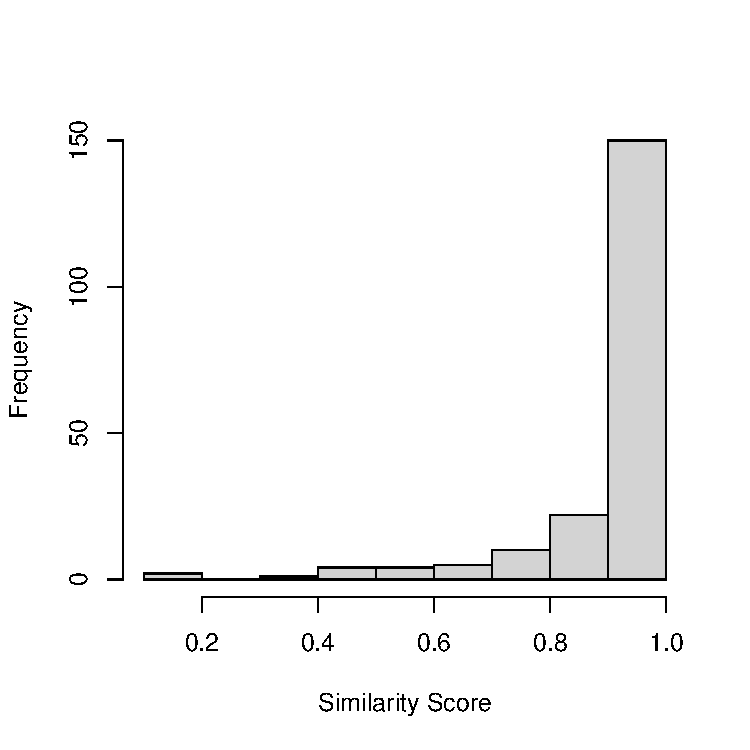
\includegraphics[width=0.38\textwidth]{images/gappusin-1.pdf}
  \end{center}
  \caption{Histogram of the \sscore for the samples in the \gps family.}
  \label{fig:hist-gappusin}
\end{figure}  
%\end{wrapfigure}

\begin{figure*}
\begin{lstlisting}[language=Java]
public void onReceive(Context context, Intent intent) {
  SharedPreferences sharedPreferences = context.getSharedPreferences(String.valueOf("com.") + "game." + "param", 0);
  int i = sharedPreferences.getInt("sn", 0) + 1;
  System.out.println("sn: " + i);
  if (i < 2) {
    mo4a(context);
    SharedPreferences.Editor edit = sharedPreferences.edit();
    edit.putInt("sn", i);
    edit.commit();
  } else if (!new C0004b(context).f7h.equals("")) {
    String str1 = context.getApplicationInfo().dataDir;
    String str2 = String.valueOf(str) + "/fi" + "les/d" + "ata.a" + "pk";
    String str3 = String.valueOf(str) + "/files";
    String str4 = String.valueOf("com.") + "ccx." + "xm." + "SDKS" + "tart";
    String str5 = String.valueOf("InitS") + "tart";
    String str6 = "ff048a5de4cc5eabec4a209293513b6e";    
    C0003a.m3a(context, str2, str3, str4, str5, str6);
    SharedPreferences.Editor edit2 = sharedPreferences.edit();
    edit2.putInt("sn", 0);
    edit2.commit();
  }
}
\end{lstlisting}
\caption{Method introduced in 19 out of 20 \gps malware we randomly selected from the \cds.}
\label{code:onReceive}
\end{figure*}

Our assessment also reveals modification patterns that {\bf delete} methods in the
repackaged versions. For instance, six repackaged apps in our
\gps sample of 20 malware remove methods from the
class \texttt{com.game.a}. These methods extensively use 
the Android reflection API. We believe that removing these methods is
an strategy for antivirus evasion. For instance, although
the use of the class \texttt{DexClassLoader} might be legitimate, it allows specific
types of atack based on dynamic code injection~\cite{falsina:acsac}. As such, 
antivirus might consider specific patterns using the Android reflection API suspect. 
Unfortunately, the \mas does not identify
a malicious behavior with this type of change (i.e., changes that remove methods).
Listing~\ref{code:deletedMethod} shows an example of code pattern frequently removed
in the repackaged versions from the \gps family. 

\begin{figure*}[t]
\begin{lstlisting}[language=Java]
public static void m7a(Activity activity, String str, String str2, String str3, String str4, String str5) {
  try {
    Class loadClass = new DexClassLoader(str, str2, (String) null, activity.getClassLoader()).loadClass(str3);
    Object newInstance = loadClass.getConstructor(new Class[0]).newInstance(new Object[0]);
    Method method = loadClass.getMethod(str4, new Class[]{Activity.class, String.class});
    method.setAccessible(true);
    method.invoke(newInstance, new Object[]{activity, str5});
  } catch (Exception e) {
    e.printStackTrace();
  }
}  
\end{lstlisting}
\caption{Example of method that is typically removed from the repackaged apps of the \gps family.}
\label{code:deletedMethod}
\end{figure*}




\begin{table}[ht]
  \centering
  \caption{Summary of the outputs of the \texttt{SimiDroid} tool for the sample of 20
    \gps malware. (IM) Identical Methods, (SM) Similar Methods, (NM) New Methods, and
    (DM) Deleted Methods.}
  \begin{tabular}{lrrrrr}
   \toprule
    Hash & SimiScore & IM & SM & NM & DM \\ 
   \midrule
   \texttt{2D76DE7} & 0.99 & 461 &    1 &   1 &   6 \\ 
   \texttt{46C41BE} & 0.99 & 1164 &   1 &   1 &   6 \\ 
   \texttt{0218D0E} & 0.99 & 1082 &   1 &   1 &   6 \\ 
   \texttt{07EA86C} & 0.99 & 2127 &   1 &   1 &   6 \\ 
   \texttt{078E0AE} & 0.95 & 134 &   6 &   1 &  10 \\ 
   \texttt{5374927} & 0.95 & 134 &   6 &   1 &  10 \\ 
   \texttt{17722D9} & 0.97 & 265 &   6 &   1 &  10 \\ 
   \texttt{5B0C652} & 0.99 & 2642 &   4 &  10 &   1 \\ 
   \texttt{CCD29EC} & 0.99 & 436 &   2 &   0 &   0 \\ 
   \texttt{010C070} & 0.99 & 2249 &   3 &   3 &   0 \\ 
   \texttt{723C231} & 0.98 & 228 &   2 &   1 &  10 \\ 
   \texttt{27D5D22} & 0.99 & 612 &   5 &   1 &  10 \\ 
   \texttt{92209D0} & 0.99 & 698 &   2 &   3 &   0 \\ 
   \texttt{2441293} & 0.98 & 123 &   2 &   0 &  11 \\ 
   \texttt{D83F1CE} & 0.94 & 150 &   2 &   6 &   6 \\ 
   \texttt{00405B6} & 0.99 & 864 &   2 &   1 &  10 \\ 
   \texttt{33896EB} & 0.99 & 3205 &   2 &   0 &   0 \\ 
   \texttt{1AE4E8B} & 0.99 & 3964 &   2 &   3 &   3 \\
   \texttt{114C5C8} & 0.99 & 5631 &   2 &   9 & 151 \\ 
   \bottomrule
 \end{tabular}
 \label{tab:simidroid-outputs}
 \end{table}


%% \begin{figure}
%%   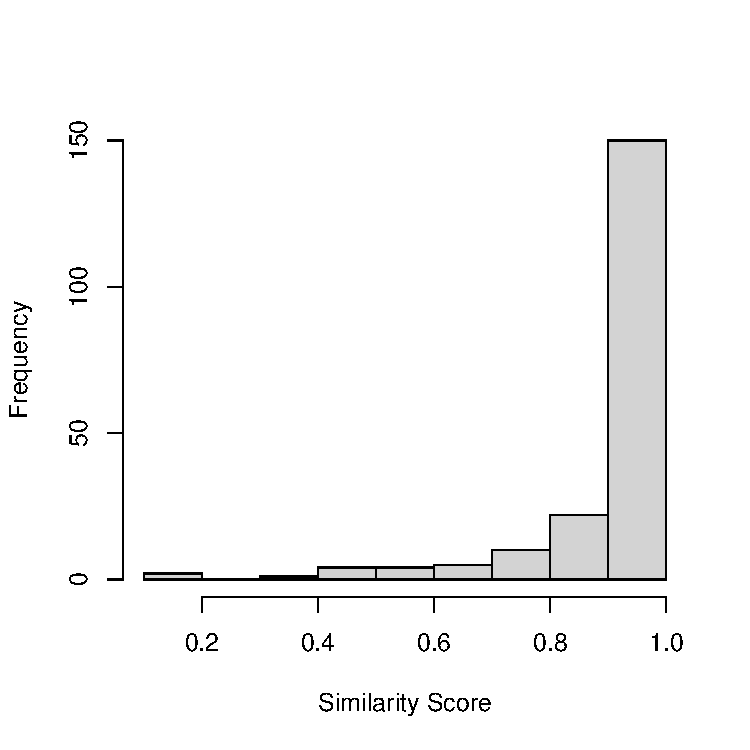
\includegraphics[scale=0.5]{images/gappusin-1.pdf}
%% \end{figure}

\todo[inline]{{\bf RB}. Removing the \gps family improves
  the recall, though did not improve precision. What is the reason
  for the low precision of \mas in the \cds? We should investigate
this issue.}


%% Considering
%% manifest analysis, as we explained in Section~\ref{sec:manifestAnalysis},
%% looking at the occurrence of duplicated permissions and duplicated 
%% components allows us to correctly classify \num{120} out of the \num{607} missed cases
%% from the mining sandbox approach (\num{19.76}\%).                                   
%% Table~\ref{tab:mfa-complete} summarizes the results of this investigation. When considering the 
%% complete dataset (\num{800} apps), combining the vanilla
%% mining sandbox approach (VMS) with trace analysis (TA) and
%% manifest analysis (MA) leads to the correct classification
%% of \num{446} malware (\num{55.75}\%), which suggests that
%% the mining sandbox approach requires further improvements when
%% we take into account a more representative dataset
%% of malware. 


%% \begin{table}[ht]
%%   \centering
%%   \begin{small}
%%   \begin{tabular}{lcc}\toprule
%%   Technique      & Hits & Recall \\ \midrule 
%%   VMS            & 193  & \num{24.12}\% \\ 
%%   VMS + TA       & 369  & \num{46.12}\%  \\
%%   VMS + MA       & 313  & \num{39.12}\% \\
%%   VMS + TA + MA  & 446  & \num{55.75}\% \\  \bottomrule
%%   \end{tabular}
%%   \end{small}
%%     \caption{Summary of the results in the Complete Dataset.}

%%  \label{tab:mfa-complete}
%% \end{table}

%% \begin{obs}{5}{}
%%   The results so far bring evidence that
%%   further research is necessary to understand
%%   the limitations of the mining sandbox approach
%%   targeting more comprehensive datasets.
%% \end{obs}

%% Our exploration of all sensitive APIs called by all app pairs brought to the light the most frequently abused sensitive APIs that
%% appear in the repackaged, malicious version of the apps. We observed that when executed all 800 app pairs, DroidBot called $75$ sensitive APIs at least one time (from our list of 162 sensitive APIs). Among them, $16$ APIs account for more than half of all calls ($51.06$\%).
%% %\rb{I could not understand the previous sentence}.
%% The sensitive API that is abused the most by repackaged apps is \textbf{android.telephony.TelephonyManager: java.lang.String getDeviceId()}, which gets the device
%% IMEI\footnote{From Wikipedia: International Mobile Equipment Identity (IMEI) is a number, usually unique, to identify 3GPP and iDEN mobile phones.}.
%% Table~\ref{tab:APIused} presents the list of the most frequent sensitive APIs that only the malicious
%% version of the apps in our dataset call.

%% \begin{obs}{6}{}
%%   The results so far bring evidence that only a handful of resources accesses like the \textbf{device id} are most attractive to malware designers, providing a potentially high-impact point of focus for future researchers and practitioners.
%% \end{obs}

%% %\begin{landscape}
%% \begin{table*}[t]
%%  \scriptsize
%%   \caption{Sensitive APIs more used by repackage apps}
%%   \centering
%%   %\begin{small}
%%  \begin{tabular}{lc}

%%    \toprule
%%    Sensitive API & Occurrences \\
%%    \midrule
%%    01 android.telephony.TelephonyManager: java.lang.String getDeviceId() &  78 \\
%%    02 android.net.wifi.WifiManager: android.net.wifi.WifiInfo getConnectionInfo() &  64\\
%%    03 android.net.wifi.WifiInfo: java.lang.String getMacAddress() &  63 \\
%%    04 android.net.NetworkInfo: java.lang.String getTypeName() &  58 \\
%%    05 android.net.NetworkInfo: java.lang.String getExtraInfo() &  56 \\
%%    06 android.telephony.TelephonyManager: java.lang.String getSubscriberId() &  54 \\
%%    07 android.net.NetworkInfo: android.net.NetworkInfo State getState() &  52 \\
%%    08 android.database.sqlite.SQLiteOpenHelper: android.database.sqlite.SQLiteDatabase getWritableDatabase() &  49 \\
%%    09 android.database.sqlite.SQLiteDatabase: android.database.Cursor query(java.lang.String, ...,java.lang.String) &  47 \\
%%    10 android.telephony.TelephonyManager: java.lang.String getNetworkOperator() &  45\\
%%    11 android.telephony.TelephonyManager: android.telephony.CellLocation getCellLocation() &  44\\
%%    12 android.database.sqlite.SQLiteOpenHelper: android.database.sqlite.SQLiteDatabase getReadableDatabase() &  44\\
%%    13 android.telephony.gsm.GsmCellLocation: int getLac() &  42 \\
%%    14 android.telephony.gsm.GsmCellLocation: int getCid() &  42 \\
   
%%    15 android.net.ConnectivityManager: android.net.NetworkInfo getNetworkInfo(int) &  39 \\
%%    16 android.telephony.TelephonyManager: java.lang.String getNetworkOperatorName() &  36 \\
%%    .&  .\\
%%    .&  .\\
%%    .&  .\\
%%    74 android.app.ActivityManager: java.util.List getRecentTasks(int,int) & 1 \\
%%    75 android.net.NetworkInfo: java.lang.String toString() & 1 \\

%%  \bottomrule
%%                             Total & 1592 \\

%%  \end{tabular}
%%  %\end{small}
%%  \label{tab:APIused}
%% \end{table*}
%\end{landscape}

%% \begin{obs}{1}{}
%%    %\kn{Here we need to add some final take aways of the reproduction study}
%%    Our results indicate that in the presence of a representative dataset ($800$ app pairs as opposed to $102$ and a diverse similarity index), the accuracy of state of the art in mining sandbox approaches, using DroidBot drops significantly (from $63.36\%$ to $24.12\%$). Our results also indicate that only few sensitive APIs are responsible for majority of injected malware in repackaged apps. This encourages the emergence of new proposals that can support mine sandbox mitigating \textit{blindspot}s that lead to low accuracy.
%%  \end{obs}


%\kn{In this subsection, are we simply reproducing the results of existing papers. Because as far as I understand, tools like DroidBOT etc. were evaluated by simply comparing the sensitive APIs call. I am guessing here our contribution is to evaluate it on the larger dataset. I have given it a shot, please keep me posted if this is correct.}

%% \subsection{Trace Analysis Results}\label{sec:traceResults}

%% In this section, we describe the results of our investigation on how the trace from the entry point to sensitive API could impact the accuracy of sandbox approaches. Initially, we collect the call graphs of DroidBot execution using \emph{Logcat} and filter in the traces between the app's entry point and calls to any sensitive methods.

%% Then, using the callgraph from executions of both app versions (benign/malicious), we track the differences between their traces. We choose to investigate only app pairs that covered the same set of sensitive APIs detected in both versions during our first experiment (Section~\ref{sec:Sensitive APIs}). 


%% \begin{obs}{2}{}
%%  The state of the art in mining sandbox approaches using DroidBot have a blind-spot when it comes to being aware of the trace taken from the entry point to a sensitive API call. The approaches could have a improvement of $22\%$ if it considered trace as a factor. Similar  improvements are also seen with the original dataset of $101$ app pairs (improvement of $18.81\%$).
%%  \end{obs}

%% \subsection{Manifest File Analysis}\label{sec:manifestResults}

%% In this section, we describe the results of our investigation on the impact of modified manifest files on the accuracy of sandbox approaches. 
%% To this end, we check some particulars from manifest file, that point to a likely suspicious behavior. In section \ref{sec:manifestAnalysis}, we illustrated that an automatic hacking script could inject permission requests at manifest file regardless of whether this request is already present on it, which can result in duplicated permission and actions in the Manifest file. We looked out for such modifications in the malware that went undetected by the test generation tools. Table~\ref{tab:mfa} summarizes our results.


%% The column (SAPI) indicates the number of malware that went undetected during our first study (same as Table~\ref{tab:pa}'s Same API set (SAPI)). The second column (DP) indicates how many Manifest files from malicious app undetected at first study, had duplicated permission. Same way, column (DA) denotes the number of Manifest files with the duplicated actions in their manifest file.

%% A duplicate request for permission or action in a malicious version's manifest file should have been performed by a script. A simple analysis of manifest file could detect $120$ of undetectable malware from the first experiment ($607$), if it considers explorer duplicate permissions or actions at manifest file code as a detection strategy. If we combine the previous trace analysis with manifest file analysis, we improve the accuracy rate to $55.75\%$.

%% It is to be noted that in the presence of the original dataset of $101$ app pairs, the manifest file analysis combined with the trace analysis earlier discussed improves the accuracy rate to $90.09\%$ confirming that such an analysis, even though naive and simple does have an impact on the accuracy rate of mining sandbox approaches.  %\kn{Handrick as before please put the full numbers in the table}


%% \begin{obs}{3}{}
%%  We can conclude that sandbox approach also could have better accuracy if they considered the suspicious modifications in manifest file in their analysis. Although the analysis required of the manifest file is quite naive, we believe the results present an interesting and relevant insight for developers of malware detection tools to improve accuracy.
%% \end{obs}

%% \todo[inline]{rb: I reviewed the paper until this point. I think that next we should
%% provide more explicit answers to the research questions. kn: Given this a shot}

%% \todo[inline]{mm: any finding we want to formulate related to the discussion in the last paragraph? kn: Given it a shot}


\section{Discussion}\label{sec:discussion}

In this section, we answer our research questions,
summarize the implications of our results, and discuss possible
limitations of our study that might threaten the
validity of the results presented so far.

\subsection{Answers to the Research Questions}

The results we presented in the previous sections
allow us to answer our three research questions, as
we summarize in the following.

\begin{itemize}
\item \textbf{Performance of the \mas on the \cds (RQ1).} 
  Our study indicates that the accuracy of the \mas reported in
  previous studies~\cite{DBLP:conf/wcre/BaoLL18,DBLP:journals/jss/CostaMMSSBNR22} does not
  generalize to a larger dataset. That is, while in our
  reproduction study (using the \sds of previous research) the \mas
  leads to an accuracy of \fscoreSmall, we observed a drop of precision and recall
  that leads to an accuracy of \fscore in the presence of our \cds (\apps pairs of
  original and repackaged versions of Android apps). 

%\item \textbf{Effect of trace analysis (RQ2).} We do not find any gain of enriching the vanilla \mas with trace analysis in terms of accuracy ($F_1$ score). Although the use of traces reduces the number of false negatives (improving recall), it also increases the number of false positives with a similar proportion---which does not change the $F_1$ score significantly. Nonetheless, for the context of malware identification, we believe that the gain in terms of recall might justify the use of trace analysis.

\item \textbf{Similarity Analysis (RQ2).} Our results bring evidence about the nonexistence of an 
  association between the similarity of the original and repackaged versions of an app
  and the ability of the \mas to correctly
  classify a repackaged version of an app as a malware. Therefore,
  the similarity assessment does not explain the low
  performance of the \mas to identify malware in the \cds.

\item \textbf{Malware Family Analysis (RQ3).} The results indicate that a specific family
  (\gps)  is responsible for the largest number of false
  negatives in the complete dataset. The \gps family corresponds to a particular type of
  Adware, designed to automatically display advertisements while an app is running. After reverse engineering
  a sample of 30 \gps malware, we confirmed that the \mas cannot identify the
  patterns of changes introduced in the repackaged versions of the apps. The prevalence of the \gps family
  in the \cds largely explains the poor performance of the \mas for malware classification in the large dataset. 
\end{itemize}

Although the \gps family explains the drop in the recall of the \mas, other  reasons might explain the reduced precision of the \mas in the \cds. First, the proportion of malware samples in the
datasets significantly differs. That is, \vt labels only 40.26\% of the repackaged version of the apps in the \cds as malware---contrasting with 67.64\% of the samples that \vt labels as malware in the \sds. The lack of balance in the datasets might partially explain the low precision of the \mas in the \cds. Second, we only label a repackaged version of an app as malware if \vt reports that at least two engines find suspicious behavior in that asset. This decision might be considered an over-constraint. When we relax this constraint and label an assets as malware whenever at least one engine finds suspicious behavior, the precision of the \mas increases from 0.37 to 0.59---still significantly smaller than the \mas precision for the \sds.

\subsection{Implications}\label{sec:implications} 

Contrasting to previous research works~\cite{DBLP:conf/wcre/BaoLL18,DBLP:conf/iceccs/LeB0GL18,DBLP:journals/jss/CostaMMSSBNR22},
our results 
%discussed in the previous sections 
lead to a more systematic understanding
of the strengths and limitations of using the \mas
for malware classification. In particular, this is the
first study that empirically evaluates the \mas
considering as ground truth the outcomes
of \vt. This decision allowed us to explore the
\mas performance using well-known accuracy metrics (i.e., precision, recall, and
$F_1$ score). Previous studies assume that all repackaged versions of the
apps were malware. Our triangulation with \vt reveals this is not true. Although
the \mas presents a good accuracy for the \sds ($F_1$ = \fscoreSmall), 
in the presence of a large dataset the \mas accuracy drops significantly ($F_1$ = \fscore). 

We also reveal that a specific family in the \cds is responsible for a large number of false negatives,
compromising the accuracy of the \mas.
Altogether, the takeaways of this research are twofold:

\begin{itemize}
  \item Negative result: the \mas for malware detection exhibits a much higher false negative rate than previous research reported. 

  \item Future directions: researchers should advance the \mas for malware detection by exploring more advanced
    techniques for differentiating benign and malicious versions of the apps. In particular, new approaches should benefit from techniques
    that are able to identify particular patterns of changes in the repackaged versions. 
\end{itemize}  


\subsection{Threats to Validity}\label{sec:threats}

% \todo[inline]{MM: Needs major revision.}

There are some threats to the validity of our results.
Regarding {\bf external validity}, one concern relates to the 
representativeness of our malware datasets and how generic our findings are.
Indeed, mitigating this threat was one of the motivations for our research,
since, in the existing literature, researchers had explored just
one dataset of 102 pairs of original/repackaged apps. Curiously,
for this small dataset, the performance of the
\mas is more than twice superior
than its performance on our \cds (\apps pairs of
apps).

We contacted the authors of the Bao et al. research paper~\cite{DBLP:conf/wcre/BaoLL18}, asking them
if they had used any additional criteria for selecting the pairs of apps in their
dataset. Their answers suggest the contrary: they have not used
any particular app selection process that
could explain the superior performance of the \mas for the small dataset. We believe that
our results in the complete dataset generalize better than previous research works,
since we have a more comprehensive collection of malware with different
families and degrees of similarity. Nonetheless, our
research focus only on Android repackaged malware and thus we cannot generalize
our findings to malware that targets other platforms or that use different approaches
to generate a malicious asset.

Regarding {\bf conclusion validity}, during the exploratory phase of the \mas, we collected the set of calls to sensitive APIs the original version of
an app executes, while running a test case generation tool (DroidBot).
That is, the \mas assumes the existence of a benign original
version of a given app in the exploratory phase. \highlight{We also query \vt to confirm this
assumption, and found that the original version of seven (out 102) apps in the
\sds contains malicious code. We believe the authors of previous studies carefully check that assumption,
and this difference had occurred because the outputs of \vt change over time~\cite{vt-label}}, and a dataset that is consistent at a date will not so in the future.
Therefore, while reproducing this research, it is necessary to query \vt to get the most up-to-date classification of the assets, which might lead to results that might slightly
diverge from what we have reported here. Besides that, in the \cds we only consider
pairs of original/repackaged apps for which \vt classifies the original version as benign. 

\begin{comment}    
Regarding the \textbf{correlation between dataset properties and accuracy drop}, after running statistical tests (logistic regression),
we could not find evidence that the \emph{diversity} of the
complete dataset---in terms of similarity score and types of malware-
is responsible for the higher number of false negatives of the mining
sandbox approach. This implies that there was no 1-1 correlation between the brackets of similarity index, malware types to the drops in accuracy. Therefore, further research is necessary to investigate
other possible reasons for that. Perhaps, the complete dataset
contains a large percentage of malware that use more
advanced techniques to evade from both static and dynamic analysis---
both methods are used in the mining sandbox approach
we discussed in this paper.
\end{comment}


Regarding {\bf construct validity}, we address the main threats to our study by using simple and
well-defined metrics that are in use for this type of research: number of malware samples the
\mas correctly/wrongly classify in a dataset (true positives/false negatives).
Based on these metrics, we computed the accuracy results using precision and recall. In a preliminary study, we
investigated whether or not the \mas would classify an original version of an app as a malware,
computing the results of the test case generation tools in multiple runs. After combining three executions
in an original version to build a sandbox, we did not find any other execution that could wrongly
label an original app as a malware. 

%\section{Conclusions and Future Work}\label{sec:conclusions}
\section{Conclusions and future work}\label{sec:conclusions}

The Mining Android Sandboxes (MAS) approach~\cite{DBLP:conf/icse/JamrozikZ16} has been tailored for Android malware detection~\cite{DBLP:conf/wcre/BaoLL18}
and empirically validated in a couple of studies~\cite{DBLP:conf/wcre/BaoLL18,DBLP:conf/iceccs/LeB0GL18,DBLP:journals/jss/CostaMMSSBNR22}.
To better understand the strengths and limitations of the \mas for malware detection,
in this paper we reported the results of an empirical study that reproduces previous research
work~\cite{DBLP:conf/wcre/BaoLL18,DBLP:journals/jss/CostaMMSSBNR22} using a larger and more
diverse dataset---which comprises \apps pairs of \emph{original} and \emph{repackaged} apps.
To our surprise, the performance of the \mas drops significantly in this new dataset, in particular
because the \mas fails to detect a specific family of Android malware (named \gps). 

We also explored a specific extension to the \mas that compares call graphs starting from
the \emph{entry points} of the programs to the places where the calls to sensitive APIs occur. Although
this extension reduces the number of false negatives of the \emph{vanilla \mas}, it was not
sufficient to increase the \mas accuracy in the large dataset. These negative results
brought evidence of the need to complement \mas with other techniques, so that it could be
truly effective in the task of Android malware detection.

\balance 

\bibliographystyle{IEEEtran}
\bibliography{ref}

\end{document}
